\documentclass[twoside]{book}

% Packages required by doxygen
\usepackage{fixltx2e}
\usepackage{calc}
\usepackage{doxygen}
\usepackage[export]{adjustbox} % also loads graphicx
\usepackage{graphicx}
\usepackage[utf8]{inputenc}
\usepackage{makeidx}
\usepackage{multicol}
\usepackage{multirow}
\PassOptionsToPackage{warn}{textcomp}
\usepackage{textcomp}
\usepackage[nointegrals]{wasysym}
\usepackage[table]{xcolor}

% Font selection
\usepackage[T1]{fontenc}
\usepackage[scaled=.90]{helvet}
\usepackage{courier}
\usepackage{amssymb}
\usepackage{sectsty}
\renewcommand{\familydefault}{\sfdefault}
\allsectionsfont{%
  \fontseries{bc}\selectfont%
  \color{darkgray}%
}
\renewcommand{\DoxyLabelFont}{%
  \fontseries{bc}\selectfont%
  \color{darkgray}%
}
\newcommand{\+}{\discretionary{\mbox{\scriptsize$\hookleftarrow$}}{}{}}

% Page & text layout
\usepackage{geometry}
\geometry{%
  a4paper,%
  top=2.5cm,%
  bottom=2.5cm,%
  left=2.5cm,%
  right=2.5cm%
}
\tolerance=750
\hfuzz=15pt
\hbadness=750
\setlength{\emergencystretch}{15pt}
\setlength{\parindent}{0cm}
\setlength{\parskip}{0.2cm}
\makeatletter
\renewcommand{\paragraph}{%
  \@startsection{paragraph}{4}{0ex}{-1.0ex}{1.0ex}{%
    \normalfont\normalsize\bfseries\SS@parafont%
  }%
}
\renewcommand{\subparagraph}{%
  \@startsection{subparagraph}{5}{0ex}{-1.0ex}{1.0ex}{%
    \normalfont\normalsize\bfseries\SS@subparafont%
  }%
}
\makeatother

% Headers & footers
\usepackage{fancyhdr}
\pagestyle{fancyplain}
\fancyhead[LE]{\fancyplain{}{\bfseries\thepage}}
\fancyhead[CE]{\fancyplain{}{}}
\fancyhead[RE]{\fancyplain{}{\bfseries\leftmark}}
\fancyhead[LO]{\fancyplain{}{\bfseries\rightmark}}
\fancyhead[CO]{\fancyplain{}{}}
\fancyhead[RO]{\fancyplain{}{\bfseries\thepage}}
\fancyfoot[LE]{\fancyplain{}{}}
\fancyfoot[CE]{\fancyplain{}{}}
\fancyfoot[RE]{\fancyplain{}{\bfseries\scriptsize Generated on Tue Aug 18 2015 12\+:12\+:11 for James Gouin et la Banane Sacrée by Doxygen }}
\fancyfoot[LO]{\fancyplain{}{\bfseries\scriptsize Generated on Tue Aug 18 2015 12\+:12\+:11 for James Gouin et la Banane Sacrée by Doxygen }}
\fancyfoot[CO]{\fancyplain{}{}}
\fancyfoot[RO]{\fancyplain{}{}}
\renewcommand{\footrulewidth}{0.4pt}
\renewcommand{\chaptermark}[1]{%
  \markboth{#1}{}%
}
\renewcommand{\sectionmark}[1]{%
  \markright{\thesection\ #1}%
}

% Indices & bibliography
\usepackage{natbib}
\usepackage[titles]{tocloft}
\setcounter{tocdepth}{3}
\setcounter{secnumdepth}{5}
\makeindex

% Hyperlinks (required, but should be loaded last)
\usepackage{ifpdf}
\ifpdf
  \usepackage[pdftex,pagebackref=true]{hyperref}
\else
  \usepackage[ps2pdf,pagebackref=true]{hyperref}
\fi
\hypersetup{%
  colorlinks=true,%
  linkcolor=blue,%
  citecolor=blue,%
  unicode%
}

% Custom commands
\newcommand{\clearemptydoublepage}{%
  \newpage{\pagestyle{empty}\cleardoublepage}%
}


%===== C O N T E N T S =====

\begin{document}

% Titlepage & ToC
\hypersetup{pageanchor=false,
             bookmarks=true,
             bookmarksnumbered=true,
             pdfencoding=unicode
            }
\pagenumbering{roman}
\begin{titlepage}
\vspace*{7cm}
\begin{center}%
{\Large James Gouin et la Banane Sacrée \\[1ex]\large Version 2.\+0 }\\
\vspace*{1cm}
{\large Generated by Doxygen 1.8.9.1}\\
\vspace*{0.5cm}
{\small Tue Aug 18 2015 12:12:11}\\
\end{center}
\end{titlepage}
\clearemptydoublepage
\tableofcontents
\clearemptydoublepage
\pagenumbering{arabic}
\hypersetup{pageanchor=true}

%--- Begin generated contents ---
\chapter{James Gouin et la Banane Sacrée}
\label{index}\hypertarget{index}{}F\+R\+A\+N\+C\+A\+I\+S\+: Jeu d’infiltration en 2\+D sans combats sous forme de puzzle game. Le joueur manipule un pingouin agent-\/secret envoyé sur un iceberg pour récupérer la « banane sacrée » volée par un singe. Son personnage peut marcher et glisser dans les quatre directions. Il fera face à un niveau de tutoriel, 6 niveaux normaux et un niveau final. Il a pour objectif de récupérer des blocs de glace auprès du boss normal de chaque niveau afin de se créer un passage jusqu’à l’iceberg central abritant l’igloo du singe. Pour cela, le joueur devra résoudre des problèmes logiques en se frayant un chemin tout en évitant d’entrer dans le champs de vision des ennemis.

E\+N\+G\+L\+I\+S\+H\+: 2\+D infiltration puzzle game without fights. The player plays at penguin character, which is a special agent sent on an iceberg to retrive the \char`\"{}holy banana\char`\"{} which was stolen by a monkey. The penguin can walk and slide in four directions. He will have to beat 8 levels including the tutorial and the final. He has as objective to retrive special ice blocks on mini bosses at the end of each level. Those blocks unlock a road to the last level in the middle of the iceberg, where the final boss is waiting. To win those blocks the player will have to solve logical problems and find his way out of the level while avoiding enemies\textquotesingle{} field of view. 

~\newline
 
\chapter{Todo List}
\label{todo}
\hypertarget{todo}{}

\begin{DoxyRefList}
\item[\label{todo__todo000001}%
\hypertarget{todo__todo000001}{}%
Class \hyperlink{class_b___movable}{B\+\_\+\+Movable} ]integrate with D\+P Factory 

integrate with D\+P Factory  
\item[\label{todo__todo000002}%
\hypertarget{todo__todo000002}{}%
Class \hyperlink{class_b___wall}{B\+\_\+\+Wall} ]integrate with D\+P Factory 

integrate with D\+P Factory  
\item[\label{todo__todo000003}%
\hypertarget{todo__todo000003}{}%
Class \hyperlink{class_b___water}{B\+\_\+\+Water} ]integrate with D\+P Factory 

integrate with D\+P Factory  
\item[\label{todo__todo000004}%
\hypertarget{todo__todo000004}{}%
Class \hyperlink{class_e___loup}{E\+\_\+\+Loup} ]integrate with D\+P Factory 

integrate with D\+P Factory  
\item[\label{todo__todo000005}%
\hypertarget{todo__todo000005}{}%
Class \hyperlink{class_e___renard}{E\+\_\+\+Renard} ]integrate with D\+P Factory 

integrate with D\+P Factory  
\item[\label{todo__todo000006}%
\hypertarget{todo__todo000006}{}%
Class \hyperlink{class_ennemi}{Ennemi} ]integrate with D\+P Factory 

integrate with D\+P Factory  
\item[\label{todo__todo000010}%
\hypertarget{todo__todo000010}{}%
Class \hyperlink{class_gameboard}{Gameboard} ]create a translation file 

create a translation file  
\item[\label{todo__todo000026}%
\hypertarget{todo__todo000026}{}%
Class \hyperlink{class_level}{Level} ]stop reading line by line  
\item[\label{todo__todo000008}%
\hypertarget{todo__todo000008}{}%
Class \hyperlink{class_m___pause}{M\+\_\+\+Pause} ]add credits 

cheat codes 

add credits 

cheat codes  
\item[\label{todo__todo000029}%
\hypertarget{todo__todo000029}{}%
Class \hyperlink{class_main_game}{Main\+Game} ]Manage the close event correctly, because it\textquotesingle{}s painful when just in the \hyperlink{class_menu_start}{Menu\+Start}.  
\item[\label{todo__todo000013}%
\hypertarget{todo__todo000013}{}%
Class \hyperlink{class_menu_start}{Menu\+Start} ]encrypt save files 

add credits 

encrypt save files 

add credits  
\item[\label{todo__todo000030}%
\hypertarget{todo__todo000030}{}%
Class \hyperlink{class_observables_ennemis}{Observables\+Ennemis} ]add management of State pattern, remplace timer by thread in \char`\"{}\+Ennemi\char`\"{}  D\+E\+L\+E\+T\+E and C\+R\+E\+A\+T\+E un new Observable\+Ennemis for the next level ! Observable\+Ennemis will delete all the enemy of the level automaticaly  
\item[\label{todo__todo000014}%
\hypertarget{todo__todo000014}{}%
Class \hyperlink{class_s___view_transition}{S\+\_\+\+View\+Transition} ]refactor into s\+\_\+door 

refactor into s\+\_\+door  
\item[\label{todo__todo000009}%
\hypertarget{todo__todo000009}{}%
Class \hyperlink{structslide_bloc}{slide\+Bloc} ]integrate with D\+P Factory 

integrate with D\+P Factory 
\end{DoxyRefList}
\chapter{Hierarchical Index}
\section{Class Hierarchy}
This inheritance list is sorted roughly, but not completely, alphabetically\+:\begin{DoxyCompactList}
\item \contentsline{section}{Factory\+\_\+\+Surface}{\pageref{class_factory___surface}}{}
\item \contentsline{section}{G\+\_\+\+Level}{\pageref{class_g___level}}{}
\item \contentsline{section}{G\+\_\+\+Profil}{\pageref{class_g___profil}}{}
\item \contentsline{section}{Observer\+\_\+\+N\+P\+C}{\pageref{class_observer___n_p_c}}{}
\item Q\+Graphics\+Item\begin{DoxyCompactList}
\item \contentsline{section}{G\+\_\+\+Character}{\pageref{class_g___character}}{}
\begin{DoxyCompactList}
\item \contentsline{section}{C\+\_\+\+Enemy}{\pageref{class_c___enemy}}{}
\begin{DoxyCompactList}
\item \contentsline{section}{E\+\_\+\+Fox}{\pageref{class_e___fox}}{}
\item \contentsline{section}{E\+\_\+\+Wolf}{\pageref{class_e___wolf}}{}
\end{DoxyCompactList}
\item \contentsline{section}{C\+\_\+\+Player}{\pageref{class_c___player}}{}
\begin{DoxyCompactList}
\item \contentsline{section}{P\+\_\+\+Penguin}{\pageref{class_p___penguin}}{}
\end{DoxyCompactList}
\end{DoxyCompactList}
\end{DoxyCompactList}
\item Q\+Graphics\+Rect\+Item\begin{DoxyCompactList}
\item \contentsline{section}{G\+\_\+\+Surface}{\pageref{class_g___surface}}{}
\begin{DoxyCompactList}
\item \contentsline{section}{B\+\_\+\+Movable}{\pageref{class_b___movable}}{}
\item \contentsline{section}{B\+\_\+\+Wall}{\pageref{class_b___wall}}{}
\item \contentsline{section}{B\+\_\+\+Water}{\pageref{class_b___water}}{}
\item \contentsline{section}{G\+\_\+\+Object}{\pageref{class_g___object}}{}
\item \contentsline{section}{S\+\_\+\+Dialog}{\pageref{class_s___dialog}}{}
\item \contentsline{section}{S\+\_\+\+Door}{\pageref{class_s___door}}{}
\item \contentsline{section}{S\+\_\+\+Ice}{\pageref{class_s___ice}}{}
\item \contentsline{section}{S\+\_\+\+Snow}{\pageref{class_s___snow}}{}
\item \contentsline{section}{S\+\_\+\+View\+Block\+N\+P\+C}{\pageref{class_s___view_block_n_p_c}}{}
\end{DoxyCompactList}
\end{DoxyCompactList}
\item Q\+Widget\begin{DoxyCompactList}
\item \contentsline{section}{G\+\_\+\+Gameboard}{\pageref{class_g___gameboard}}{}
\item \contentsline{section}{G\+\_\+\+Main\+Game}{\pageref{class_g___main_game}}{}
\item \contentsline{section}{W\+\_\+\+Dialog}{\pageref{class_w___dialog}}{}
\item \contentsline{section}{W\+\_\+\+Life}{\pageref{class_w___life}}{}
\item \contentsline{section}{W\+\_\+\+Menu\+Pause}{\pageref{class_w___menu_pause}}{}
\item \contentsline{section}{W\+\_\+\+Menu\+Start}{\pageref{class_w___menu_start}}{}
\item \contentsline{section}{W\+\_\+\+Object}{\pageref{class_w___object}}{}
\end{DoxyCompactList}
\item \contentsline{section}{Sliding\+Block}{\pageref{struct_sliding_block}}{}
\item \contentsline{section}{State\+\_\+\+Enemy}{\pageref{class_state___enemy}}{}
\begin{DoxyCompactList}
\item \contentsline{section}{State\+\_\+\+Enemy\+Patrol}{\pageref{class_state___enemy_patrol}}{}
\item \contentsline{section}{State\+\_\+\+Enemy\+Sleep}{\pageref{class_state___enemy_sleep}}{}
\end{DoxyCompactList}
\item \contentsline{section}{State\+\_\+\+Enemy\+Pause}{\pageref{class_state___enemy_pause}}{}
\end{DoxyCompactList}

\chapter{Class Index}
\section{Class List}
Here are the classes, structs, unions and interfaces with brief descriptions\+:\begin{DoxyCompactList}
\item\contentsline{section}{\hyperlink{class_b___movable}{B\+\_\+\+Movable} \\*Movable block }{\pageref{class_b___movable}}{}
\item\contentsline{section}{\hyperlink{class_b___wall}{B\+\_\+\+Wall} }{\pageref{class_b___wall}}{}
\item\contentsline{section}{\hyperlink{class_b___water}{B\+\_\+\+Water} }{\pageref{class_b___water}}{}
\item\contentsline{section}{\hyperlink{class_e___loup}{E\+\_\+\+Loup} }{\pageref{class_e___loup}}{}
\item\contentsline{section}{\hyperlink{class_e___renard}{E\+\_\+\+Renard} \\*Enemy Character\+: Fox }{\pageref{class_e___renard}}{}
\item\contentsline{section}{\hyperlink{class_ennemi}{Ennemi} \\*Enemy Class }{\pageref{class_ennemi}}{}
\item\contentsline{section}{\hyperlink{class_gameboard}{Gameboard} \\*Game Board. Where the game happens }{\pageref{class_gameboard}}{}
\item\contentsline{section}{\hyperlink{class_level}{Level} }{\pageref{class_level}}{}
\item\contentsline{section}{\hyperlink{class_m___pause}{M\+\_\+\+Pause} }{\pageref{class_m___pause}}{}
\item\contentsline{section}{\hyperlink{class_main_game}{Main\+Game} \\*Q\+Widget principal gerant le programme du jeu dans le fond }{\pageref{class_main_game}}{}
\item\contentsline{section}{\hyperlink{class_menu_start}{Menu\+Start} \\*Premier menu (start) que le joueur voie en lancant le jeu }{\pageref{class_menu_start}}{}
\item\contentsline{section}{\hyperlink{class_object}{Object} }{\pageref{class_object}}{}
\item\contentsline{section}{\hyperlink{class_pingouin}{Pingouin} }{\pageref{class_pingouin}}{}
\item\contentsline{section}{\hyperlink{class_player}{Player} }{\pageref{class_player}}{}
\item\contentsline{section}{\hyperlink{class_profil}{Profil} }{\pageref{class_profil}}{}
\item\contentsline{section}{\hyperlink{class_s___dialog}{S\+\_\+\+Dialog} }{\pageref{class_s___dialog}}{}
\item\contentsline{section}{\hyperlink{class_s___ice}{S\+\_\+\+Ice} }{\pageref{class_s___ice}}{}
\item\contentsline{section}{\hyperlink{class_s___snow}{S\+\_\+\+Snow} }{\pageref{class_s___snow}}{}
\item\contentsline{section}{\hyperlink{class_s___view_bloc_ennemi}{S\+\_\+\+View\+Bloc\+Ennemi} }{\pageref{class_s___view_bloc_ennemi}}{}
\item\contentsline{section}{\hyperlink{class_s___view_transition}{S\+\_\+\+View\+Transition} }{\pageref{class_s___view_transition}}{}
\item\contentsline{section}{\hyperlink{structslide_bloc}{slide\+Bloc} }{\pageref{structslide_bloc}}{}
\item\contentsline{section}{\hyperlink{class_surface}{Surface} }{\pageref{class_surface}}{}
\item\contentsline{section}{\hyperlink{class_widget_dialog}{Widget\+Dialog} }{\pageref{class_widget_dialog}}{}
\item\contentsline{section}{\hyperlink{class_widget_life}{Widget\+Life} }{\pageref{class_widget_life}}{}
\item\contentsline{section}{\hyperlink{class_widget_object}{Widget\+Object} }{\pageref{class_widget_object}}{}
\end{DoxyCompactList}

\chapter{Class Documentation}
\hypertarget{class_b___movable}{}\section{B\+\_\+\+Movable Class Reference}
\label{class_b___movable}\index{B\+\_\+\+Movable@{B\+\_\+\+Movable}}


Movable block.  




{\ttfamily \#include $<$b\+\_\+movable.\+h$>$}

Inheritance diagram for B\+\_\+\+Movable\+:\begin{figure}[H]
\begin{center}
\leavevmode
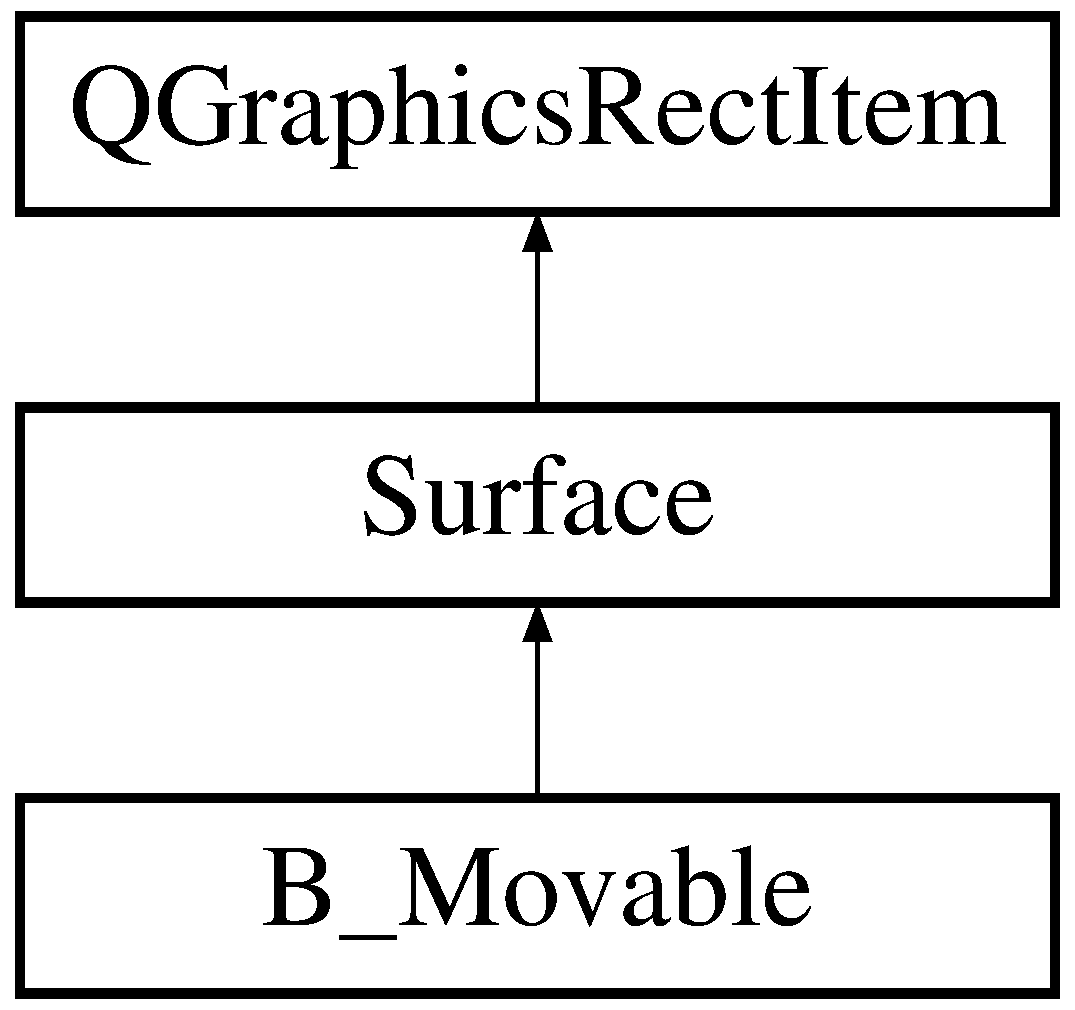
\includegraphics[height=3.000000cm]{class_b___movable}
\end{center}
\end{figure}
\subsection*{Public Member Functions}
\begin{DoxyCompactItemize}
\item 
\hyperlink{class_b___movable_ac874fc12d19502117d0bfc396d1059d2}{B\+\_\+\+Movable} (int xpos, int ypos, Q\+Graphics\+Item $\ast$parent=0)
\begin{DoxyCompactList}\small\item\em Constructor with position setup. \end{DoxyCompactList}\item 
\hyperlink{class_b___movable_aef88fa8933731c08731796a9ee3fda6b}{B\+\_\+\+Movable} (Q\+Graphics\+Item $\ast$parent=0)
\begin{DoxyCompactList}\small\item\em Constructor without position setup. \end{DoxyCompactList}\item 
void \hyperlink{class_b___movable_a8a23ac4b1692d95607dcccd6d6c9a973}{add\+To\+Scene} (Q\+Graphics\+Scene $\ast$Scene)
\begin{DoxyCompactList}\small\item\em Add self to scene. \end{DoxyCompactList}\item 
void \hyperlink{class_b___movable_aa4d26e877655021ef70bc6914fe04418}{remove\+From\+Scene} (Q\+Graphics\+Scene $\ast$Scene)
\begin{DoxyCompactList}\small\item\em Remove self to scene. \end{DoxyCompactList}\item 
void \hyperlink{class_b___movable_a55fb8069fc55c4edabd2ac076acdee17}{move\+By} (int x, int y)
\begin{DoxyCompactList}\small\item\em Move self by x and y values. \end{DoxyCompactList}\item 
void \hyperlink{class_b___movable_aca717ec608426940422f1bc658201bf5}{set\+Pos} (int x, int y)
\begin{DoxyCompactList}\small\item\em Set the position of self with the x and y values. \end{DoxyCompactList}\item 
bool \hyperlink{class_b___movable_a5d28eb38771a241e59a403876670fa52}{is\+Movable\+To\+Left} ()
\begin{DoxyCompactList}\small\item\em Check if self can move to the left. \end{DoxyCompactList}\item 
bool \hyperlink{class_b___movable_a36fab7cd8d7d7d6d026d054512c10929}{is\+Movable\+To\+Right} ()
\begin{DoxyCompactList}\small\item\em Check if self can move to the right. \end{DoxyCompactList}\item 
bool \hyperlink{class_b___movable_a4b9fda4b276b9d9448bcc9e8feec6cb5}{is\+Movable\+To\+Bottom} ()
\begin{DoxyCompactList}\small\item\em Check if self can move to the bottom. \end{DoxyCompactList}\item 
bool \hyperlink{class_b___movable_acdd4c8c72909da2994e79dff5f24f71b}{is\+Movable\+To\+Top} ()
\begin{DoxyCompactList}\small\item\em Check if self can move to the top. \end{DoxyCompactList}\item 
bool \hyperlink{class_b___movable_a44d1413ec8bceda3b1a50c673b429d03}{is\+Slide} ()
\begin{DoxyCompactList}\small\item\em Check if self should slide. \end{DoxyCompactList}\item 
Q\+List$<$ Q\+Graphics\+Item $\ast$ $>$ \hyperlink{class_b___movable_ab597ec57dd4bfed453d5e329a2b82990}{collides\+Center} ()
\begin{DoxyCompactList}\small\item\em Get all colliding blocks. \end{DoxyCompactList}\item 
Q\+Graphics\+Rect\+Item $\ast$ \hyperlink{class_b___movable_a4cb26e3d494505eaaa6773c0a448c479}{get\+Collide\+Bloc\+Position} (char sens)
\begin{DoxyCompactList}\small\item\em Get the colliding block from a direction. \end{DoxyCompactList}\end{DoxyCompactItemize}
\subsection*{Public Attributes}
\begin{DoxyCompactItemize}
\item 
\hypertarget{class_b___movable_ab838f983e5e7b13148fc7f4873f2c347}{}Q\+Graphics\+Rect\+Item $\ast$ \hyperlink{class_b___movable_ab838f983e5e7b13148fc7f4873f2c347}{left\+Collide\+Box}\label{class_b___movable_ab838f983e5e7b13148fc7f4873f2c347}

\begin{DoxyCompactList}\small\item\em Box on the left side of the b\+\_\+movable. \end{DoxyCompactList}\item 
\hypertarget{class_b___movable_a5da8e8b462e4504f219857a3e007ad97}{}Q\+Graphics\+Rect\+Item $\ast$ \hyperlink{class_b___movable_a5da8e8b462e4504f219857a3e007ad97}{right\+Collide\+Box}\label{class_b___movable_a5da8e8b462e4504f219857a3e007ad97}

\begin{DoxyCompactList}\small\item\em Box on the right side of the b\+\_\+movable. \end{DoxyCompactList}\item 
\hypertarget{class_b___movable_a6ad546481827dc987708ad36023ba21b}{}Q\+Graphics\+Rect\+Item $\ast$ \hyperlink{class_b___movable_a6ad546481827dc987708ad36023ba21b}{bottom\+Collide\+Box}\label{class_b___movable_a6ad546481827dc987708ad36023ba21b}

\begin{DoxyCompactList}\small\item\em Box on the bottom side of the b\+\_\+movable. \end{DoxyCompactList}\item 
\hypertarget{class_b___movable_a0609a13a4c686a8c7a4a0edb5e87efbf}{}Q\+Graphics\+Rect\+Item $\ast$ \hyperlink{class_b___movable_a0609a13a4c686a8c7a4a0edb5e87efbf}{top\+Collide\+Box}\label{class_b___movable_a0609a13a4c686a8c7a4a0edb5e87efbf}

\begin{DoxyCompactList}\small\item\em Box on the top side of the b\+\_\+movable. \end{DoxyCompactList}\end{DoxyCompactItemize}


\subsection{Detailed Description}
Movable block. 

This block can be moved with characters. \begin{DoxyAuthor}{Author}
Claret Romain, \href{mailto:romain.claret@rocla.ch}{\tt romain.\+claret@rocla.\+ch} 

Divernois Margaux, \href{mailto:margaux.divernois@gmail.com}{\tt margaux.\+divernois@gmail.\+com} 

Visinand Steve, \href{mailto:visinandst@gmail.com}{\tt visinandst@gmail.\+com} 
\end{DoxyAuthor}
\begin{DoxyCopyright}{Copyright}
Custom License + N\+D\+A 
\end{DoxyCopyright}
\begin{DoxyVersion}{Version}
1.\+0 
\end{DoxyVersion}
\begin{DoxyDate}{Date}
27 January 2015 
\end{DoxyDate}
\begin{DoxyRefDesc}{Todo}
\item[\hyperlink{todo__todo000001}{Todo}]integrate with D\+P Factory \end{DoxyRefDesc}


\subsection{Constructor \& Destructor Documentation}
\hypertarget{class_b___movable_ac874fc12d19502117d0bfc396d1059d2}{}\index{B\+\_\+\+Movable@{B\+\_\+\+Movable}!B\+\_\+\+Movable@{B\+\_\+\+Movable}}
\index{B\+\_\+\+Movable@{B\+\_\+\+Movable}!B\+\_\+\+Movable@{B\+\_\+\+Movable}}
\subsubsection[{B\+\_\+\+Movable}]{\setlength{\rightskip}{0pt plus 5cm}B\+\_\+\+Movable\+::\+B\+\_\+\+Movable (
\begin{DoxyParamCaption}
\item[{int}]{xpos, }
\item[{int}]{ypos, }
\item[{Q\+Graphics\+Item $\ast$}]{parent = {\ttfamily 0}}
\end{DoxyParamCaption}
)}\label{class_b___movable_ac874fc12d19502117d0bfc396d1059d2}


Constructor with position setup. 


\begin{DoxyParams}{Parameters}
{\em xpos} & set the postion on the x-\/axis \\
\hline
{\em ypos} & set the postion on the y-\/axis \\
\hline
{\em parent} & Q\+Graphics\+Item parent\\
\hline
\end{DoxyParams}
Uses set\+Design(xpos, ypos) to create the cross of box around self to check collisions. Sets the position on the Z-\/axis to 1 to be on top of the scene which is at 0. \hypertarget{class_b___movable_aef88fa8933731c08731796a9ee3fda6b}{}\index{B\+\_\+\+Movable@{B\+\_\+\+Movable}!B\+\_\+\+Movable@{B\+\_\+\+Movable}}
\index{B\+\_\+\+Movable@{B\+\_\+\+Movable}!B\+\_\+\+Movable@{B\+\_\+\+Movable}}
\subsubsection[{B\+\_\+\+Movable}]{\setlength{\rightskip}{0pt plus 5cm}B\+\_\+\+Movable\+::\+B\+\_\+\+Movable (
\begin{DoxyParamCaption}
\item[{Q\+Graphics\+Item $\ast$}]{parent = {\ttfamily 0}}
\end{DoxyParamCaption}
)}\label{class_b___movable_aef88fa8933731c08731796a9ee3fda6b}


Constructor without position setup. 


\begin{DoxyParams}{Parameters}
{\em parent} & Q\+Graphics\+Item to depend on\\
\hline
\end{DoxyParams}
The use F\+I\+C\+T\+I\+V\+E positions x and y to create the cross of box around self to check collisions. Sets the position on the Z-\/axis to 1 to be on top of the scene which is at 0. 

\subsection{Member Function Documentation}
\hypertarget{class_b___movable_a8a23ac4b1692d95607dcccd6d6c9a973}{}\index{B\+\_\+\+Movable@{B\+\_\+\+Movable}!add\+To\+Scene@{add\+To\+Scene}}
\index{add\+To\+Scene@{add\+To\+Scene}!B\+\_\+\+Movable@{B\+\_\+\+Movable}}
\subsubsection[{add\+To\+Scene}]{\setlength{\rightskip}{0pt plus 5cm}void B\+\_\+\+Movable\+::add\+To\+Scene (
\begin{DoxyParamCaption}
\item[{Q\+Graphics\+Scene $\ast$}]{Scene}
\end{DoxyParamCaption}
)}\label{class_b___movable_a8a23ac4b1692d95607dcccd6d6c9a973}


Add self to scene. 


\begin{DoxyParams}{Parameters}
{\em Scene} & scene to add self to\\
\hline
\end{DoxyParams}
Add self and the cross for colliding detectection. \hypertarget{class_b___movable_ab597ec57dd4bfed453d5e329a2b82990}{}\index{B\+\_\+\+Movable@{B\+\_\+\+Movable}!collides\+Center@{collides\+Center}}
\index{collides\+Center@{collides\+Center}!B\+\_\+\+Movable@{B\+\_\+\+Movable}}
\subsubsection[{collides\+Center}]{\setlength{\rightskip}{0pt plus 5cm}Q\+List$<$ Q\+Graphics\+Item $\ast$ $>$ B\+\_\+\+Movable\+::collides\+Center (
\begin{DoxyParamCaption}
{}
\end{DoxyParamCaption}
)}\label{class_b___movable_ab597ec57dd4bfed453d5e329a2b82990}


Get all colliding blocks. 

\begin{DoxyReturn}{Returns}
colliding Q\+Graphics\+Item 
\end{DoxyReturn}
\hypertarget{class_b___movable_a4cb26e3d494505eaaa6773c0a448c479}{}\index{B\+\_\+\+Movable@{B\+\_\+\+Movable}!get\+Collide\+Bloc\+Position@{get\+Collide\+Bloc\+Position}}
\index{get\+Collide\+Bloc\+Position@{get\+Collide\+Bloc\+Position}!B\+\_\+\+Movable@{B\+\_\+\+Movable}}
\subsubsection[{get\+Collide\+Bloc\+Position}]{\setlength{\rightskip}{0pt plus 5cm}Q\+Graphics\+Rect\+Item $\ast$ B\+\_\+\+Movable\+::get\+Collide\+Bloc\+Position (
\begin{DoxyParamCaption}
\item[{char}]{sens}
\end{DoxyParamCaption}
)}\label{class_b___movable_a4cb26e3d494505eaaa6773c0a448c479}


Get the colliding block from a direction. 


\begin{DoxyParams}{Parameters}
{\em sens} & the side to check for a collision \\
\hline
\end{DoxyParams}
\begin{DoxyReturn}{Returns}
Q\+Graphics\+Rect\+Item in collision with the parameter
\end{DoxyReturn}
Check the direction as parameter (\char`\"{}b\char`\"{}\+:bottom,\char`\"{}l\char`\"{}\+:left,\char`\"{}r\char`\"{}\+:right,\char`\"{}t\char`\"{}\+:top). Return N\+U\+L\+L if no colliding item is found. \hypertarget{class_b___movable_a4b9fda4b276b9d9448bcc9e8feec6cb5}{}\index{B\+\_\+\+Movable@{B\+\_\+\+Movable}!is\+Movable\+To\+Bottom@{is\+Movable\+To\+Bottom}}
\index{is\+Movable\+To\+Bottom@{is\+Movable\+To\+Bottom}!B\+\_\+\+Movable@{B\+\_\+\+Movable}}
\subsubsection[{is\+Movable\+To\+Bottom}]{\setlength{\rightskip}{0pt plus 5cm}bool B\+\_\+\+Movable\+::is\+Movable\+To\+Bottom (
\begin{DoxyParamCaption}
{}
\end{DoxyParamCaption}
)}\label{class_b___movable_a4b9fda4b276b9d9448bcc9e8feec6cb5}


Check if self can move to the bottom. 

\begin{DoxyReturn}{Returns}
true if can move to bottom 
\end{DoxyReturn}
\hypertarget{class_b___movable_a5d28eb38771a241e59a403876670fa52}{}\index{B\+\_\+\+Movable@{B\+\_\+\+Movable}!is\+Movable\+To\+Left@{is\+Movable\+To\+Left}}
\index{is\+Movable\+To\+Left@{is\+Movable\+To\+Left}!B\+\_\+\+Movable@{B\+\_\+\+Movable}}
\subsubsection[{is\+Movable\+To\+Left}]{\setlength{\rightskip}{0pt plus 5cm}bool B\+\_\+\+Movable\+::is\+Movable\+To\+Left (
\begin{DoxyParamCaption}
{}
\end{DoxyParamCaption}
)}\label{class_b___movable_a5d28eb38771a241e59a403876670fa52}


Check if self can move to the left. 

\begin{DoxyReturn}{Returns}
true if can move to left 
\end{DoxyReturn}
\hypertarget{class_b___movable_a36fab7cd8d7d7d6d026d054512c10929}{}\index{B\+\_\+\+Movable@{B\+\_\+\+Movable}!is\+Movable\+To\+Right@{is\+Movable\+To\+Right}}
\index{is\+Movable\+To\+Right@{is\+Movable\+To\+Right}!B\+\_\+\+Movable@{B\+\_\+\+Movable}}
\subsubsection[{is\+Movable\+To\+Right}]{\setlength{\rightskip}{0pt plus 5cm}bool B\+\_\+\+Movable\+::is\+Movable\+To\+Right (
\begin{DoxyParamCaption}
{}
\end{DoxyParamCaption}
)}\label{class_b___movable_a36fab7cd8d7d7d6d026d054512c10929}


Check if self can move to the right. 

\begin{DoxyReturn}{Returns}
true if can move to right 
\end{DoxyReturn}
\hypertarget{class_b___movable_acdd4c8c72909da2994e79dff5f24f71b}{}\index{B\+\_\+\+Movable@{B\+\_\+\+Movable}!is\+Movable\+To\+Top@{is\+Movable\+To\+Top}}
\index{is\+Movable\+To\+Top@{is\+Movable\+To\+Top}!B\+\_\+\+Movable@{B\+\_\+\+Movable}}
\subsubsection[{is\+Movable\+To\+Top}]{\setlength{\rightskip}{0pt plus 5cm}bool B\+\_\+\+Movable\+::is\+Movable\+To\+Top (
\begin{DoxyParamCaption}
{}
\end{DoxyParamCaption}
)}\label{class_b___movable_acdd4c8c72909da2994e79dff5f24f71b}


Check if self can move to the top. 

\begin{DoxyReturn}{Returns}
true if can move to top 
\end{DoxyReturn}
\hypertarget{class_b___movable_a44d1413ec8bceda3b1a50c673b429d03}{}\index{B\+\_\+\+Movable@{B\+\_\+\+Movable}!is\+Slide@{is\+Slide}}
\index{is\+Slide@{is\+Slide}!B\+\_\+\+Movable@{B\+\_\+\+Movable}}
\subsubsection[{is\+Slide}]{\setlength{\rightskip}{0pt plus 5cm}bool B\+\_\+\+Movable\+::is\+Slide (
\begin{DoxyParamCaption}
{}
\end{DoxyParamCaption}
)}\label{class_b___movable_a44d1413ec8bceda3b1a50c673b429d03}


Check if self should slide. 

\begin{DoxyReturn}{Returns}
true if self collides with a specific block.
\end{DoxyReturn}
Check if the cross of detection collides with \hyperlink{class_s___ice}{S\+\_\+\+Ice}. \hypertarget{class_b___movable_a55fb8069fc55c4edabd2ac076acdee17}{}\index{B\+\_\+\+Movable@{B\+\_\+\+Movable}!move\+By@{move\+By}}
\index{move\+By@{move\+By}!B\+\_\+\+Movable@{B\+\_\+\+Movable}}
\subsubsection[{move\+By}]{\setlength{\rightskip}{0pt plus 5cm}void B\+\_\+\+Movable\+::move\+By (
\begin{DoxyParamCaption}
\item[{int}]{x, }
\item[{int}]{y}
\end{DoxyParamCaption}
)}\label{class_b___movable_a55fb8069fc55c4edabd2ac076acdee17}


Move self by x and y values. 


\begin{DoxyParams}{Parameters}
{\em x} & move this amount on the x-\/axis \\
\hline
{\em y} & move this amount on the y-\/axis\\
\hline
\end{DoxyParams}
Move self and the cross for colliding detectection. \hypertarget{class_b___movable_aa4d26e877655021ef70bc6914fe04418}{}\index{B\+\_\+\+Movable@{B\+\_\+\+Movable}!remove\+From\+Scene@{remove\+From\+Scene}}
\index{remove\+From\+Scene@{remove\+From\+Scene}!B\+\_\+\+Movable@{B\+\_\+\+Movable}}
\subsubsection[{remove\+From\+Scene}]{\setlength{\rightskip}{0pt plus 5cm}void B\+\_\+\+Movable\+::remove\+From\+Scene (
\begin{DoxyParamCaption}
\item[{Q\+Graphics\+Scene $\ast$}]{Scene}
\end{DoxyParamCaption}
)}\label{class_b___movable_aa4d26e877655021ef70bc6914fe04418}


Remove self to scene. 


\begin{DoxyParams}{Parameters}
{\em Scene} & scene to remove self from\\
\hline
\end{DoxyParams}
Remove self and the cross for colliding detectection. \hypertarget{class_b___movable_aca717ec608426940422f1bc658201bf5}{}\index{B\+\_\+\+Movable@{B\+\_\+\+Movable}!set\+Pos@{set\+Pos}}
\index{set\+Pos@{set\+Pos}!B\+\_\+\+Movable@{B\+\_\+\+Movable}}
\subsubsection[{set\+Pos}]{\setlength{\rightskip}{0pt plus 5cm}void B\+\_\+\+Movable\+::set\+Pos (
\begin{DoxyParamCaption}
\item[{int}]{x, }
\item[{int}]{y}
\end{DoxyParamCaption}
)}\label{class_b___movable_aca717ec608426940422f1bc658201bf5}


Set the position of self with the x and y values. 


\begin{DoxyParams}{Parameters}
{\em x} & set the postion on the x-\/axis \\
\hline
{\em y} & set the postion on the y-\/axis \\
\hline
\end{DoxyParams}


The documentation for this class was generated from the following files\+:\begin{DoxyCompactItemize}
\item 
b\+\_\+movable.\+h\item 
b\+\_\+movable.\+cpp\end{DoxyCompactItemize}

\hypertarget{class_b___wall}{}\section{B\+\_\+\+Wall Class Reference}
\label{class_b___wall}\index{B\+\_\+\+Wall@{B\+\_\+\+Wall}}


Wall block.  




{\ttfamily \#include $<$b\+\_\+wall.\+h$>$}

Inheritance diagram for B\+\_\+\+Wall\+:\begin{figure}[H]
\begin{center}
\leavevmode
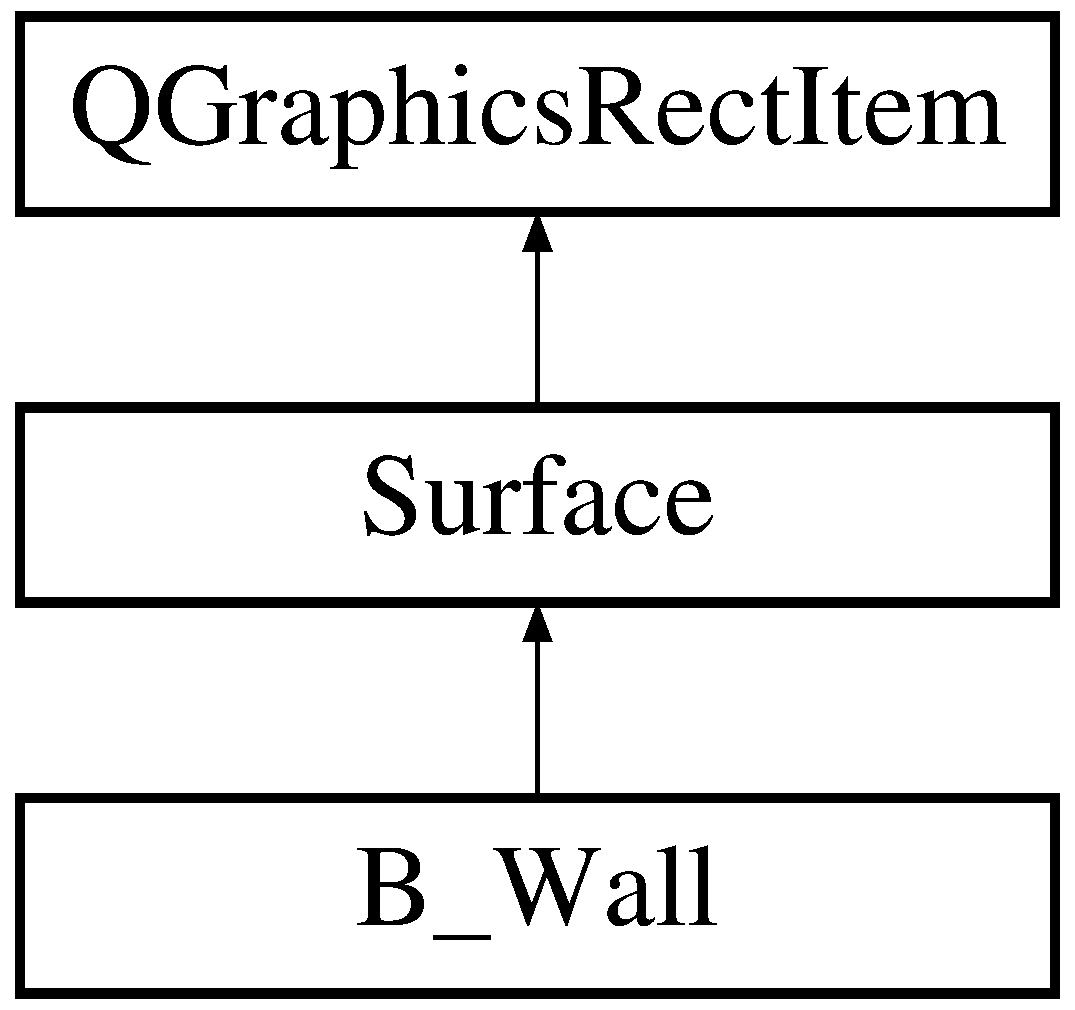
\includegraphics[height=3.000000cm]{class_b___wall}
\end{center}
\end{figure}
\subsection*{Public Member Functions}
\begin{DoxyCompactItemize}
\item 
\hyperlink{class_b___wall_ad83db8883f6d620be7f9430b962c5774}{B\+\_\+\+Wall} (int xpos, int ypos, Q\+Graphics\+Item $\ast$parent=0)
\begin{DoxyCompactList}\small\item\em Constructor with position setup. \end{DoxyCompactList}\item 
\hyperlink{class_b___wall_a04cf7394644c9ca59a21e0e4dc1e63a6}{B\+\_\+\+Wall} (Q\+Graphics\+Item $\ast$parent=0)
\begin{DoxyCompactList}\small\item\em Constructor without position setup. \end{DoxyCompactList}\end{DoxyCompactItemize}


\subsection{Detailed Description}
Wall block. 

This block can not be moved with characters. \begin{DoxyAuthor}{Author}
Claret Romain, \href{mailto:romain.claret@rocla.ch}{\tt romain.\+claret@rocla.\+ch} 

Divernois Margaux, \href{mailto:margaux.divernois@gmail.com}{\tt margaux.\+divernois@gmail.\+com} 

Visinand Steve, \href{mailto:visinandst@gmail.com}{\tt visinandst@gmail.\+com} 
\end{DoxyAuthor}
\begin{DoxyCopyright}{Copyright}
Custom License + N\+D\+A 
\end{DoxyCopyright}
\begin{DoxyVersion}{Version}
1.\+0 
\end{DoxyVersion}
\begin{DoxyDate}{Date}
27 January 2015 
\end{DoxyDate}
\begin{DoxyRefDesc}{Todo}
\item[\hyperlink{todo__todo000002}{Todo}]integrate with D\+P Factory \end{DoxyRefDesc}


\subsection{Constructor \& Destructor Documentation}
\hypertarget{class_b___wall_ad83db8883f6d620be7f9430b962c5774}{}\index{B\+\_\+\+Wall@{B\+\_\+\+Wall}!B\+\_\+\+Wall@{B\+\_\+\+Wall}}
\index{B\+\_\+\+Wall@{B\+\_\+\+Wall}!B\+\_\+\+Wall@{B\+\_\+\+Wall}}
\subsubsection[{B\+\_\+\+Wall}]{\setlength{\rightskip}{0pt plus 5cm}B\+\_\+\+Wall\+::\+B\+\_\+\+Wall (
\begin{DoxyParamCaption}
\item[{int}]{xpos, }
\item[{int}]{ypos, }
\item[{Q\+Graphics\+Item $\ast$}]{parent = {\ttfamily 0}}
\end{DoxyParamCaption}
)}\label{class_b___wall_ad83db8883f6d620be7f9430b962c5774}


Constructor with position setup. 


\begin{DoxyParams}{Parameters}
{\em xpos} & set the postion on the x-\/axis \\
\hline
{\em ypos} & set the postion on the y-\/axis \\
\hline
{\em parent} & Q\+Graphics\+Item parent \\
\hline
\end{DoxyParams}
\hypertarget{class_b___wall_a04cf7394644c9ca59a21e0e4dc1e63a6}{}\index{B\+\_\+\+Wall@{B\+\_\+\+Wall}!B\+\_\+\+Wall@{B\+\_\+\+Wall}}
\index{B\+\_\+\+Wall@{B\+\_\+\+Wall}!B\+\_\+\+Wall@{B\+\_\+\+Wall}}
\subsubsection[{B\+\_\+\+Wall}]{\setlength{\rightskip}{0pt plus 5cm}B\+\_\+\+Wall\+::\+B\+\_\+\+Wall (
\begin{DoxyParamCaption}
\item[{Q\+Graphics\+Item $\ast$}]{parent = {\ttfamily 0}}
\end{DoxyParamCaption}
)}\label{class_b___wall_a04cf7394644c9ca59a21e0e4dc1e63a6}


Constructor without position setup. 


\begin{DoxyParams}{Parameters}
{\em parent} & Q\+Graphics\+Item parent\\
\hline
\end{DoxyParams}
No other choice that use F\+I\+C\+T\+I\+V\+E positions x and y. Here set at 0. 

The documentation for this class was generated from the following files\+:\begin{DoxyCompactItemize}
\item 
b\+\_\+wall.\+h\item 
b\+\_\+wall.\+cpp\end{DoxyCompactItemize}

\hypertarget{class_b___water}{}\section{B\+\_\+\+Water Class Reference}
\label{class_b___water}\index{B\+\_\+\+Water@{B\+\_\+\+Water}}
Inheritance diagram for B\+\_\+\+Water\+:\begin{figure}[H]
\begin{center}
\leavevmode
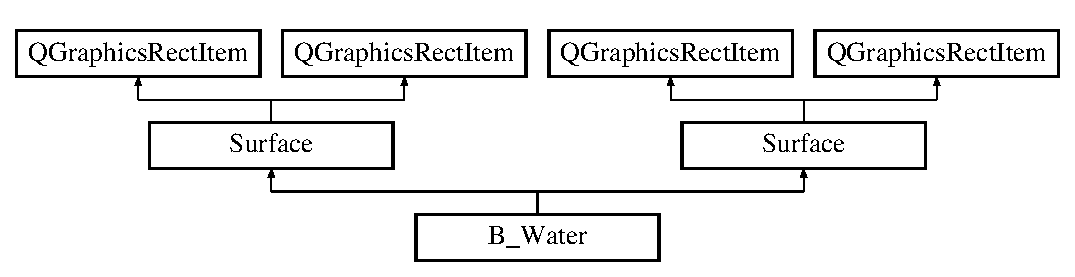
\includegraphics[height=3.000000cm]{class_b___water}
\end{center}
\end{figure}
\subsection*{Public Member Functions}
\begin{DoxyCompactItemize}
\item 
\hypertarget{class_b___water_a6c1ef8207043a950c74583332e00bb7f}{}{\bfseries B\+\_\+\+Water} (int xpos, int ypos, Q\+Graphics\+Item $\ast$parent=0)\label{class_b___water_a6c1ef8207043a950c74583332e00bb7f}

\item 
\hypertarget{class_b___water_a7286659987b70322806f866c1faaf218}{}{\bfseries B\+\_\+\+Water} (Q\+Graphics\+Item $\ast$parent=0)\label{class_b___water_a7286659987b70322806f866c1faaf218}

\end{DoxyCompactItemize}


The documentation for this class was generated from the following files\+:\begin{DoxyCompactItemize}
\item 
b\+\_\+water.\+h\item 
b\+\_\+water.\+cpp\end{DoxyCompactItemize}

\hypertarget{class_e___loup}{}\section{E\+\_\+\+Loup Class Reference}
\label{class_e___loup}\index{E\+\_\+\+Loup@{E\+\_\+\+Loup}}
Inheritance diagram for E\+\_\+\+Loup\+:\begin{figure}[H]
\begin{center}
\leavevmode
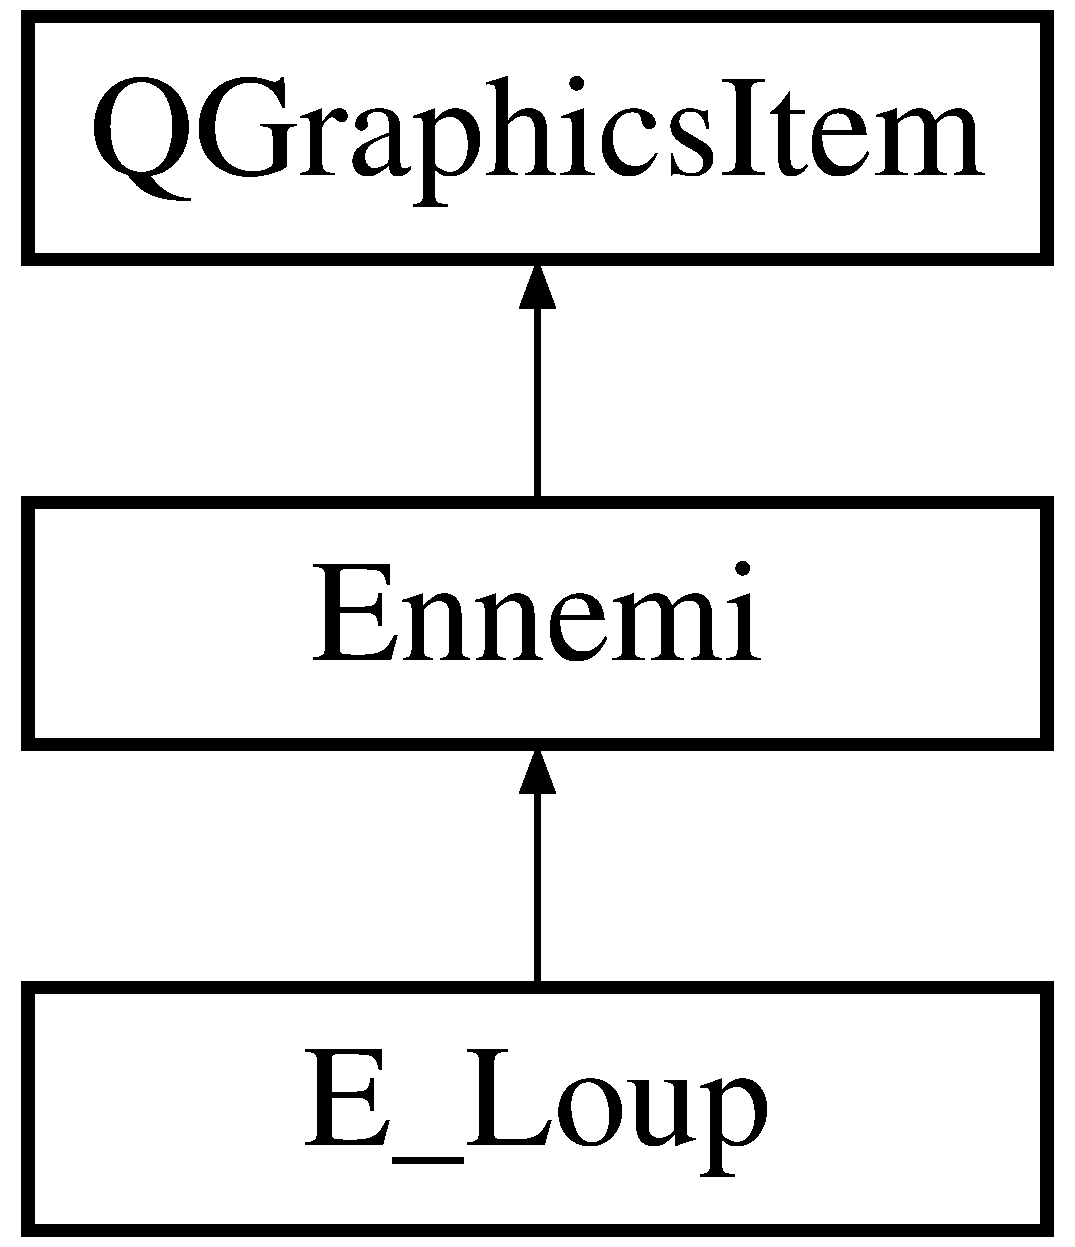
\includegraphics[height=3.000000cm]{class_e___loup}
\end{center}
\end{figure}
\subsection*{Public Member Functions}
\begin{DoxyCompactItemize}
\item 
\hypertarget{class_e___loup_a666e273642dae36a9baf98dc47ee0dc9}{}{\bfseries E\+\_\+\+Loup} (Q\+List$<$ Q\+Point $>$ path)\label{class_e___loup_a666e273642dae36a9baf98dc47ee0dc9}

\end{DoxyCompactItemize}
\subsection*{Additional Inherited Members}


The documentation for this class was generated from the following files\+:\begin{DoxyCompactItemize}
\item 
e\+\_\+loup.\+h\item 
e\+\_\+loup.\+cpp\end{DoxyCompactItemize}

\hypertarget{class_e___renard}{}\section{E\+\_\+\+Renard Class Reference}
\label{class_e___renard}\index{E\+\_\+\+Renard@{E\+\_\+\+Renard}}


Enemy Character\+: Fox.  




{\ttfamily \#include $<$e\+\_\+renard.\+h$>$}

Inheritance diagram for E\+\_\+\+Renard\+:\begin{figure}[H]
\begin{center}
\leavevmode
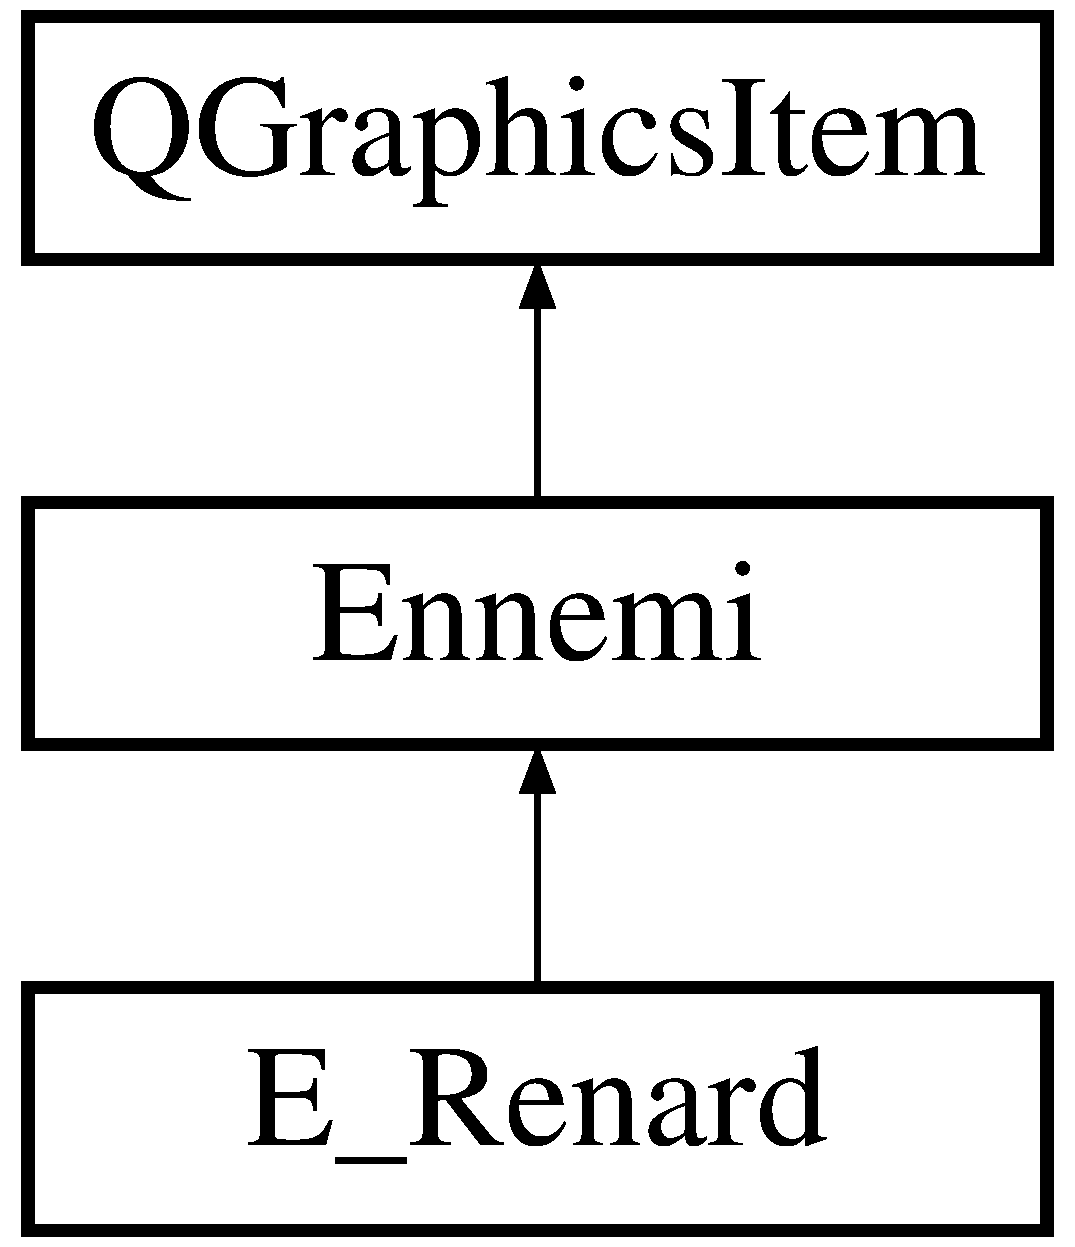
\includegraphics[height=3.000000cm]{class_e___renard}
\end{center}
\end{figure}
\subsection*{Public Member Functions}
\begin{DoxyCompactItemize}
\item 
\hyperlink{class_e___renard_aa5c7e87d02089ed76c306a3434133645}{E\+\_\+\+Renard} (Q\+List$<$ Q\+Point $>$ path, \hyperlink{class_gameboard}{Gameboard} $\ast$g)
\begin{DoxyCompactList}\small\item\em Constructor with path setup. \end{DoxyCompactList}\end{DoxyCompactItemize}
\subsection*{Additional Inherited Members}


\subsection{Detailed Description}
Enemy Character\+: Fox. 

This is a character with its own characteristics. It moves on a automatic pattern generated between two given points. His view is 3x2 blocs. \begin{DoxyAuthor}{Author}
Claret Romain, \href{mailto:romain.claret@rocla.ch}{\tt romain.\+claret@rocla.\+ch} 

Divernois Margaux, \href{mailto:margaux.divernois@gmail.com}{\tt margaux.\+divernois@gmail.\+com} 

Visinand Steve, \href{mailto:visinandst@gmail.com}{\tt visinandst@gmail.\+com} 
\end{DoxyAuthor}
\begin{DoxyCopyright}{Copyright}
Custom License + N\+D\+A 
\end{DoxyCopyright}
\begin{DoxyVersion}{Version}
1.\+0 
\end{DoxyVersion}
\begin{DoxyDate}{Date}
27 January 2015 
\end{DoxyDate}
\begin{DoxyRefDesc}{Todo}
\item[\hyperlink{todo__todo000005}{Todo}]integrate with D\+P Factory \end{DoxyRefDesc}


\subsection{Constructor \& Destructor Documentation}
\hypertarget{class_e___renard_aa5c7e87d02089ed76c306a3434133645}{}\index{E\+\_\+\+Renard@{E\+\_\+\+Renard}!E\+\_\+\+Renard@{E\+\_\+\+Renard}}
\index{E\+\_\+\+Renard@{E\+\_\+\+Renard}!E\+\_\+\+Renard@{E\+\_\+\+Renard}}
\subsubsection[{E\+\_\+\+Renard}]{\setlength{\rightskip}{0pt plus 5cm}E\+\_\+\+Renard\+::\+E\+\_\+\+Renard (
\begin{DoxyParamCaption}
\item[{Q\+List$<$ Q\+Point $>$}]{path, }
\item[{{\bf Gameboard} $\ast$}]{g}
\end{DoxyParamCaption}
)}\label{class_e___renard_aa5c7e87d02089ed76c306a3434133645}


Constructor with path setup. 


\begin{DoxyParams}{Parameters}
{\em path} & Q\+List of Q\+Point for the path \\
\hline
{\em g} & \hyperlink{class_gameboard}{Gameboard} to construct on\\
\hline
\end{DoxyParams}
Set the skin, speed at 10, Z value at 2 and default orientation to top. Vision of the enemy is created here. 

The documentation for this class was generated from the following files\+:\begin{DoxyCompactItemize}
\item 
e\+\_\+renard.\+h\item 
e\+\_\+renard.\+cpp\end{DoxyCompactItemize}

\hypertarget{class_ennemi}{}\section{Ennemi Class Reference}
\label{class_ennemi}\index{Ennemi@{Ennemi}}


Enemy Class.  




{\ttfamily \#include $<$ennemi.\+h$>$}

Inheritance diagram for Ennemi\+:\begin{figure}[H]
\begin{center}
\leavevmode
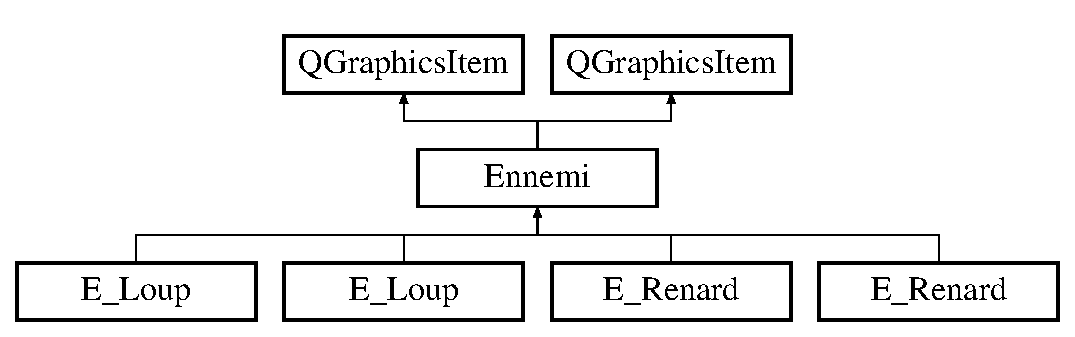
\includegraphics[height=3.000000cm]{class_ennemi}
\end{center}
\end{figure}
\subsection*{Public Member Functions}
\begin{DoxyCompactItemize}
\item 
\hyperlink{class_ennemi_af86e9134a1cfd8d878305924702b9d7a}{Ennemi} (Q\+List$<$ Q\+Point $>$, \hyperlink{class_gameboard}{Gameboard} $\ast$g)
\begin{DoxyCompactList}\small\item\em Constructor with path setup. \end{DoxyCompactList}\item 
\hypertarget{class_ennemi_adf402a9389efe705c604f91d6e74d00e}{}\hyperlink{class_ennemi_adf402a9389efe705c604f91d6e74d00e}{$\sim$\+Ennemi} ()\label{class_ennemi_adf402a9389efe705c604f91d6e74d00e}

\begin{DoxyCompactList}\small\item\em Destruction of the blocks used for the vision. \end{DoxyCompactList}\item 
\hypertarget{class_ennemi_ae62d1dcf274319710e7ac4495c95a221}{}void \hyperlink{class_ennemi_ae62d1dcf274319710e7ac4495c95a221}{add\+To\+Scene} (Q\+Graphics\+Scene $\ast$)\label{class_ennemi_ae62d1dcf274319710e7ac4495c95a221}

\begin{DoxyCompactList}\small\item\em Add self to the scene. \end{DoxyCompactList}\item 
\hypertarget{class_ennemi_aa00ff90bbb5d71456a23673e77c41bb4}{}Q\+Rect\+F {\bfseries bounding\+Rect} () const \label{class_ennemi_aa00ff90bbb5d71456a23673e77c41bb4}

\item 
\hypertarget{class_ennemi_afbdea6c2e62c2065694a32db0f049325}{}void {\bfseries paint} (Q\+Painter $\ast$painter, const Q\+Style\+Option\+Graphics\+Item $\ast$option, Q\+Widget $\ast$widget)\label{class_ennemi_afbdea6c2e62c2065694a32db0f049325}

\item 
\hypertarget{class_ennemi_a7c509f048996eecb4ee768a044825d15}{}void \hyperlink{class_ennemi_a7c509f048996eecb4ee768a044825d15}{set\+Orientation\+\_\+top} ()\label{class_ennemi_a7c509f048996eecb4ee768a044825d15}

\begin{DoxyCompactList}\small\item\em Set the orientation of self to the top. \end{DoxyCompactList}\item 
\hypertarget{class_ennemi_ab3bbc6381307320c22b1686c5bc59d93}{}void \hyperlink{class_ennemi_ab3bbc6381307320c22b1686c5bc59d93}{set\+Orientation\+\_\+bottom} ()\label{class_ennemi_ab3bbc6381307320c22b1686c5bc59d93}

\begin{DoxyCompactList}\small\item\em Set the orientation of self to the bottom. \end{DoxyCompactList}\item 
\hypertarget{class_ennemi_ac455b7c41a46dc42a27841b9c566e329}{}void \hyperlink{class_ennemi_ac455b7c41a46dc42a27841b9c566e329}{set\+Orientation\+\_\+left} ()\label{class_ennemi_ac455b7c41a46dc42a27841b9c566e329}

\begin{DoxyCompactList}\small\item\em Set the orientation of self to the left. \end{DoxyCompactList}\item 
\hypertarget{class_ennemi_a4e99225c7a632efceebba66996d7d9ee}{}void \hyperlink{class_ennemi_a4e99225c7a632efceebba66996d7d9ee}{set\+Orientation\+\_\+right} ()\label{class_ennemi_a4e99225c7a632efceebba66996d7d9ee}

\begin{DoxyCompactList}\small\item\em Set the orientation of self to the right. \end{DoxyCompactList}\item 
\hypertarget{class_ennemi_a482e9c5ccc0cf1c3aa4e83f32f3eedb1}{}void \hyperlink{class_ennemi_a482e9c5ccc0cf1c3aa4e83f32f3eedb1}{set\+Path} (Q\+List$<$ Q\+Point $>$)\label{class_ennemi_a482e9c5ccc0cf1c3aa4e83f32f3eedb1}

\begin{DoxyCompactList}\small\item\em Set the path of self for the automatic displacement. \end{DoxyCompactList}\item 
void \hyperlink{class_ennemi_a6811b0a25a92ec210750072b83d1f74e}{pinguin\+On\+View\+Bloc} ()
\begin{DoxyCompactList}\small\item\em Restart game is Playable character is detected. \end{DoxyCompactList}\item 
\hypertarget{class_ennemi_ad4861b8a3ad9d4819d3716ac3d0e8501}{}void \hyperlink{class_ennemi_ad4861b8a3ad9d4819d3716ac3d0e8501}{view\+Bloc\+Actif} ()\label{class_ennemi_ad4861b8a3ad9d4819d3716ac3d0e8501}

\begin{DoxyCompactList}\small\item\em Enable or Disable vision blocks. \end{DoxyCompactList}\item 
Q\+Point \hyperlink{class_ennemi_a14529c0dc2ad2edf3b5d174221ffa6ff}{get\+Enemy\+Pos} ()
\begin{DoxyCompactList}\small\item\em get\+Enemy\+Pos return the position with the correct coords on the map \end{DoxyCompactList}\item 
void \hyperlink{class_ennemi_a3d8cf7a7d4b577a46cfdfaa1f37e9ded}{change\+State} (\hyperlink{class_state_ennemi}{State\+Ennemi} $\ast$new\+State)
\begin{DoxyCompactList}\small\item\em change\+State replace the state of the enemy with new\+State \end{DoxyCompactList}\item 
\hyperlink{class_ennemi_af86e9134a1cfd8d878305924702b9d7a}{Ennemi} (Q\+List$<$ Q\+Point $>$, \hyperlink{class_gameboard}{Gameboard} $\ast$g)
\begin{DoxyCompactList}\small\item\em Constructor with path setup. \end{DoxyCompactList}\item 
\hypertarget{class_ennemi_adf402a9389efe705c604f91d6e74d00e}{}\hyperlink{class_ennemi_adf402a9389efe705c604f91d6e74d00e}{$\sim$\+Ennemi} ()\label{class_ennemi_adf402a9389efe705c604f91d6e74d00e}

\begin{DoxyCompactList}\small\item\em Destruction of the blocks used for the vision. \end{DoxyCompactList}\item 
\hypertarget{class_ennemi_ae62d1dcf274319710e7ac4495c95a221}{}void \hyperlink{class_ennemi_ae62d1dcf274319710e7ac4495c95a221}{add\+To\+Scene} (Q\+Graphics\+Scene $\ast$)\label{class_ennemi_ae62d1dcf274319710e7ac4495c95a221}

\begin{DoxyCompactList}\small\item\em Add self to the scene. \end{DoxyCompactList}\item 
\hypertarget{class_ennemi_aa00ff90bbb5d71456a23673e77c41bb4}{}Q\+Rect\+F {\bfseries bounding\+Rect} () const \label{class_ennemi_aa00ff90bbb5d71456a23673e77c41bb4}

\item 
\hypertarget{class_ennemi_afbdea6c2e62c2065694a32db0f049325}{}void {\bfseries paint} (Q\+Painter $\ast$painter, const Q\+Style\+Option\+Graphics\+Item $\ast$option, Q\+Widget $\ast$widget)\label{class_ennemi_afbdea6c2e62c2065694a32db0f049325}

\item 
\hypertarget{class_ennemi_a7c509f048996eecb4ee768a044825d15}{}void \hyperlink{class_ennemi_a7c509f048996eecb4ee768a044825d15}{set\+Orientation\+\_\+top} ()\label{class_ennemi_a7c509f048996eecb4ee768a044825d15}

\begin{DoxyCompactList}\small\item\em Set the orientation of self to the top. \end{DoxyCompactList}\item 
\hypertarget{class_ennemi_ab3bbc6381307320c22b1686c5bc59d93}{}void \hyperlink{class_ennemi_ab3bbc6381307320c22b1686c5bc59d93}{set\+Orientation\+\_\+bottom} ()\label{class_ennemi_ab3bbc6381307320c22b1686c5bc59d93}

\begin{DoxyCompactList}\small\item\em Set the orientation of self to the bottom. \end{DoxyCompactList}\item 
\hypertarget{class_ennemi_ac455b7c41a46dc42a27841b9c566e329}{}void \hyperlink{class_ennemi_ac455b7c41a46dc42a27841b9c566e329}{set\+Orientation\+\_\+left} ()\label{class_ennemi_ac455b7c41a46dc42a27841b9c566e329}

\begin{DoxyCompactList}\small\item\em Set the orientation of self to the left. \end{DoxyCompactList}\item 
\hypertarget{class_ennemi_a4e99225c7a632efceebba66996d7d9ee}{}void \hyperlink{class_ennemi_a4e99225c7a632efceebba66996d7d9ee}{set\+Orientation\+\_\+right} ()\label{class_ennemi_a4e99225c7a632efceebba66996d7d9ee}

\begin{DoxyCompactList}\small\item\em Set the orientation of self to the right. \end{DoxyCompactList}\item 
\hypertarget{class_ennemi_a482e9c5ccc0cf1c3aa4e83f32f3eedb1}{}void \hyperlink{class_ennemi_a482e9c5ccc0cf1c3aa4e83f32f3eedb1}{set\+Path} (Q\+List$<$ Q\+Point $>$)\label{class_ennemi_a482e9c5ccc0cf1c3aa4e83f32f3eedb1}

\begin{DoxyCompactList}\small\item\em Set the path of self for the automatic displacement. \end{DoxyCompactList}\item 
\hypertarget{class_ennemi_a6811b0a25a92ec210750072b83d1f74e}{}void \hyperlink{class_ennemi_a6811b0a25a92ec210750072b83d1f74e}{pinguin\+On\+View\+Bloc} ()\label{class_ennemi_a6811b0a25a92ec210750072b83d1f74e}

\begin{DoxyCompactList}\small\item\em Restart game is Playable character is detected. \end{DoxyCompactList}\item 
\hypertarget{class_ennemi_ad4861b8a3ad9d4819d3716ac3d0e8501}{}void \hyperlink{class_ennemi_ad4861b8a3ad9d4819d3716ac3d0e8501}{view\+Bloc\+Actif} ()\label{class_ennemi_ad4861b8a3ad9d4819d3716ac3d0e8501}

\begin{DoxyCompactList}\small\item\em Enable or Disable vision blocks. \end{DoxyCompactList}\item 
Q\+Point \hyperlink{class_ennemi_a14529c0dc2ad2edf3b5d174221ffa6ff}{get\+Enemy\+Pos} ()
\begin{DoxyCompactList}\small\item\em get\+Enemy\+Pos return the position with the correct coords on the map \end{DoxyCompactList}\item 
void \hyperlink{class_ennemi_a3d8cf7a7d4b577a46cfdfaa1f37e9ded}{change\+State} (\hyperlink{class_state_ennemi}{State\+Ennemi} $\ast$new\+State)
\begin{DoxyCompactList}\small\item\em change\+State replace the state of the enemy with new\+State \end{DoxyCompactList}\end{DoxyCompactItemize}
\subsection*{Protected Member Functions}
\begin{DoxyCompactItemize}
\item 
void \hyperlink{class_ennemi_a68785ba49227d8588b0acc1fcc9856fa}{advance} (int step)
\begin{DoxyCompactList}\small\item\em Moves self by an amount. \end{DoxyCompactList}\item 
void \hyperlink{class_ennemi_a029f6711fe3817f9697a8369718e50f6}{set\+Pos\+View\+Bloc} (\hyperlink{class_s___view_bloc_ennemi}{S\+\_\+\+View\+Bloc\+Ennemi} $\ast$bloc, Q\+Point p)
\begin{DoxyCompactList}\small\item\em Set the position of the block \char`\"{}\+S\+\_\+\+View\+Bloc\+Ennemi\char`\"{}. \end{DoxyCompactList}\item 
void \hyperlink{class_ennemi_a68785ba49227d8588b0acc1fcc9856fa}{advance} (int step)
\begin{DoxyCompactList}\small\item\em Moves self by an amount. \end{DoxyCompactList}\item 
void \hyperlink{class_ennemi_a029f6711fe3817f9697a8369718e50f6}{set\+Pos\+View\+Bloc} (\hyperlink{class_s___view_bloc_ennemi}{S\+\_\+\+View\+Bloc\+Ennemi} $\ast$bloc, Q\+Point p)
\begin{DoxyCompactList}\small\item\em Set the position of the block \char`\"{}\+S\+\_\+\+View\+Bloc\+Ennemi\char`\"{}. \end{DoxyCompactList}\end{DoxyCompactItemize}
\subsection*{Protected Attributes}
\begin{DoxyCompactItemize}
\item 
\hypertarget{class_ennemi_abf051ea1d034df4a8b0480e9387f2008}{}int {\bfseries speed}\label{class_ennemi_abf051ea1d034df4a8b0480e9387f2008}

\item 
\hypertarget{class_ennemi_acbd9a5c07e51a477a42daf0496d864e4}{}Q\+List$<$ Q\+Point $>$ {\bfseries path}\label{class_ennemi_acbd9a5c07e51a477a42daf0496d864e4}

\item 
\hypertarget{class_ennemi_a54e9c4370bff0dd2a6b05c24a4fd06f7}{}Q\+List$<$ \hyperlink{class_s___view_bloc_ennemi}{S\+\_\+\+View\+Bloc\+Ennemi} $\ast$ $>$ {\bfseries champ\+Vue}\label{class_ennemi_a54e9c4370bff0dd2a6b05c24a4fd06f7}

\item 
\hypertarget{class_ennemi_a5537ad37a49d572d09a76749238490c2}{}Q\+String {\bfseries left\+Skin}\label{class_ennemi_a5537ad37a49d572d09a76749238490c2}

\item 
\hypertarget{class_ennemi_ab63f4a7fbff796d8c368bd49e254561a}{}Q\+String {\bfseries right\+Skin}\label{class_ennemi_ab63f4a7fbff796d8c368bd49e254561a}

\item 
\hypertarget{class_ennemi_abe2b3007be5ed71b5547a66407b8db3e}{}Q\+String {\bfseries up\+Skin}\label{class_ennemi_abe2b3007be5ed71b5547a66407b8db3e}

\item 
\hypertarget{class_ennemi_a3a72c0537216823ea706923d20f9ed5a}{}Q\+String {\bfseries down\+Skin}\label{class_ennemi_a3a72c0537216823ea706923d20f9ed5a}

\item 
\hypertarget{class_ennemi_aef6146a86a5b04b34f0e7292a1ddd237}{}Q\+Brush $\ast$ {\bfseries ennemi\+Skin}\label{class_ennemi_aef6146a86a5b04b34f0e7292a1ddd237}

\end{DoxyCompactItemize}
\subsection*{Friends}
\begin{DoxyCompactItemize}
\item 
\hypertarget{class_ennemi_ad4e940eeddddccbb3f0fa1b9c6655b19}{}class {\bfseries State\+Ennemi}\label{class_ennemi_ad4e940eeddddccbb3f0fa1b9c6655b19}

\item 
\hypertarget{class_ennemi_a3993e6f153d417c1b39a3fd9887fd2fe}{}class {\bfseries State\+Ennemi\+\_\+\+Patrol}\label{class_ennemi_a3993e6f153d417c1b39a3fd9887fd2fe}

\item 
\hypertarget{class_ennemi_aabb95dc3768b5bcbfc4b8577fd2e8673}{}class {\bfseries State\+Ennemi\+\_\+\+Sleep}\label{class_ennemi_aabb95dc3768b5bcbfc4b8577fd2e8673}

\item 
\hypertarget{class_ennemi_a6a6b7120d88c0cd46c85c0af86341abf}{}class {\bfseries State\+Ennemi\+\_\+\+Pause}\label{class_ennemi_a6a6b7120d88c0cd46c85c0af86341abf}

\end{DoxyCompactItemize}


\subsection{Detailed Description}
Enemy Class. 

Parent class for enemies. Contains the orientation, the path, the skin, the definition, and the specification. \begin{DoxyAuthor}{Author}
Claret Romain, \href{mailto:romain.claret@rocla.ch}{\tt romain.\+claret@rocla.\+ch} 

Divernois Margaux, \href{mailto:margaux.divernois@gmail.com}{\tt margaux.\+divernois@gmail.\+com} 

Visinand Steve, \href{mailto:visinandst@gmail.com}{\tt visinandst@gmail.\+com} 
\end{DoxyAuthor}
\begin{DoxyCopyright}{Copyright}
Custom License + N\+D\+A 
\end{DoxyCopyright}
\begin{DoxyVersion}{Version}
1.\+0 
\end{DoxyVersion}
\begin{DoxyDate}{Date}
27 January 2015 
\end{DoxyDate}
\begin{DoxyRefDesc}{Todo}
\item[\hyperlink{todo__todo000006}{Todo}]integrate with D\+P Factory \end{DoxyRefDesc}


Parent class for enemies. Contains the orientation, the path, the skin, the definition, and the specification. \begin{DoxyAuthor}{Author}
Claret Romain, \href{mailto:romain.claret@rocla.ch}{\tt romain.\+claret@rocla.\+ch} 

Divernois Margaux, \href{mailto:margaux.divernois@gmail.com}{\tt margaux.\+divernois@gmail.\+com} 

Visinand Steve, \href{mailto:visinandst@gmail.com}{\tt visinandst@gmail.\+com} 
\end{DoxyAuthor}
\begin{DoxyCopyright}{Copyright}
Custom License + N\+D\+A 
\end{DoxyCopyright}
\begin{DoxyVersion}{Version}
1.\+0 
\end{DoxyVersion}
\begin{DoxyDate}{Date}
27 January 2015 
\end{DoxyDate}
\begin{DoxyRefDesc}{Todo}
\item[\hyperlink{todo__todo000015}{Todo}]integrate with D\+P Factory \end{DoxyRefDesc}


\subsection{Constructor \& Destructor Documentation}
\hypertarget{class_ennemi_af86e9134a1cfd8d878305924702b9d7a}{}\index{Ennemi@{Ennemi}!Ennemi@{Ennemi}}
\index{Ennemi@{Ennemi}!Ennemi@{Ennemi}}
\subsubsection[{Ennemi}]{\setlength{\rightskip}{0pt plus 5cm}Ennemi\+::\+Ennemi (
\begin{DoxyParamCaption}
\item[{Q\+List$<$ Q\+Point $>$}]{path, }
\item[{{\bf Gameboard} $\ast$}]{g}
\end{DoxyParamCaption}
)}\label{class_ennemi_af86e9134a1cfd8d878305924702b9d7a}


Constructor with path setup. 


\begin{DoxyParams}{Parameters}
{\em path} & Q\+List of Q\+Point for the path \\
\hline
{\em g} & \hyperlink{class_gameboard}{Gameboard} to depend on\\
\hline
\end{DoxyParams}
Set the speed at 100, Z value at 2, detect\+Pinguin to false, sens to true and the path given. For the speed\+: 1 is really fast, 100 is really slow. \hypertarget{class_ennemi_af86e9134a1cfd8d878305924702b9d7a}{}\index{Ennemi@{Ennemi}!Ennemi@{Ennemi}}
\index{Ennemi@{Ennemi}!Ennemi@{Ennemi}}
\subsubsection[{Ennemi}]{\setlength{\rightskip}{0pt plus 5cm}Ennemi\+::\+Ennemi (
\begin{DoxyParamCaption}
\item[{Q\+List$<$ Q\+Point $>$}]{, }
\item[{{\bf Gameboard} $\ast$}]{g}
\end{DoxyParamCaption}
)}\label{class_ennemi_af86e9134a1cfd8d878305924702b9d7a}


Constructor with path setup. 


\begin{DoxyParams}{Parameters}
{\em path} & Q\+List of Q\+Point for the path \\
\hline
{\em g} & \hyperlink{class_gameboard}{Gameboard} to depend on \\
\hline
\end{DoxyParams}


\subsection{Member Function Documentation}
\hypertarget{class_ennemi_a68785ba49227d8588b0acc1fcc9856fa}{}\index{Ennemi@{Ennemi}!advance@{advance}}
\index{advance@{advance}!Ennemi@{Ennemi}}
\subsubsection[{advance}]{\setlength{\rightskip}{0pt plus 5cm}void Ennemi\+::advance (
\begin{DoxyParamCaption}
\item[{int}]{step}
\end{DoxyParamCaption}
)\hspace{0.3cm}{\ttfamily [protected]}}\label{class_ennemi_a68785ba49227d8588b0acc1fcc9856fa}


Moves self by an amount. 


\begin{DoxyParams}{Parameters}
{\em step} & amount to move self \\
\hline
\end{DoxyParams}
\hypertarget{class_ennemi_a68785ba49227d8588b0acc1fcc9856fa}{}\index{Ennemi@{Ennemi}!advance@{advance}}
\index{advance@{advance}!Ennemi@{Ennemi}}
\subsubsection[{advance}]{\setlength{\rightskip}{0pt plus 5cm}void Ennemi\+::advance (
\begin{DoxyParamCaption}
\item[{int}]{step}
\end{DoxyParamCaption}
)\hspace{0.3cm}{\ttfamily [protected]}}\label{class_ennemi_a68785ba49227d8588b0acc1fcc9856fa}


Moves self by an amount. 


\begin{DoxyParams}{Parameters}
{\em step} & amount to move self\\
\hline
\end{DoxyParams}
Executed at each call of the slot \hyperlink{class_ennemi_a68785ba49227d8588b0acc1fcc9856fa}{advance()} from the Scene. It is the brain of the enemy. \hypertarget{class_ennemi_a3d8cf7a7d4b577a46cfdfaa1f37e9ded}{}\index{Ennemi@{Ennemi}!change\+State@{change\+State}}
\index{change\+State@{change\+State}!Ennemi@{Ennemi}}
\subsubsection[{change\+State}]{\setlength{\rightskip}{0pt plus 5cm}void Ennemi\+::change\+State (
\begin{DoxyParamCaption}
\item[{{\bf State\+Ennemi} $\ast$}]{new\+State}
\end{DoxyParamCaption}
)}\label{class_ennemi_a3d8cf7a7d4b577a46cfdfaa1f37e9ded}


change\+State replace the state of the enemy with new\+State 


\begin{DoxyParams}{Parameters}
{\em new\+State} & replace the state of the enemy with new\+State \\
\hline
\end{DoxyParams}
\hypertarget{class_ennemi_a3d8cf7a7d4b577a46cfdfaa1f37e9ded}{}\index{Ennemi@{Ennemi}!change\+State@{change\+State}}
\index{change\+State@{change\+State}!Ennemi@{Ennemi}}
\subsubsection[{change\+State}]{\setlength{\rightskip}{0pt plus 5cm}void Ennemi\+::change\+State (
\begin{DoxyParamCaption}
\item[{{\bf State\+Ennemi} $\ast$}]{new\+State}
\end{DoxyParamCaption}
)}\label{class_ennemi_a3d8cf7a7d4b577a46cfdfaa1f37e9ded}


change\+State replace the state of the enemy with new\+State 


\begin{DoxyParams}{Parameters}
{\em new\+State} & \\
\hline
\end{DoxyParams}
\hypertarget{class_ennemi_a14529c0dc2ad2edf3b5d174221ffa6ff}{}\index{Ennemi@{Ennemi}!get\+Enemy\+Pos@{get\+Enemy\+Pos}}
\index{get\+Enemy\+Pos@{get\+Enemy\+Pos}!Ennemi@{Ennemi}}
\subsubsection[{get\+Enemy\+Pos}]{\setlength{\rightskip}{0pt plus 5cm}Q\+Point Ennemi\+::get\+Enemy\+Pos (
\begin{DoxyParamCaption}
{}
\end{DoxyParamCaption}
)}\label{class_ennemi_a14529c0dc2ad2edf3b5d174221ffa6ff}


get\+Enemy\+Pos return the position with the correct coords on the map 

\begin{DoxyReturn}{Returns}
position of the enemy
\end{DoxyReturn}
get\+Enemy\+Pos return the position with the correct coords on the map \hypertarget{class_ennemi_a14529c0dc2ad2edf3b5d174221ffa6ff}{}\index{Ennemi@{Ennemi}!get\+Enemy\+Pos@{get\+Enemy\+Pos}}
\index{get\+Enemy\+Pos@{get\+Enemy\+Pos}!Ennemi@{Ennemi}}
\subsubsection[{get\+Enemy\+Pos}]{\setlength{\rightskip}{0pt plus 5cm}Q\+Point Ennemi\+::get\+Enemy\+Pos (
\begin{DoxyParamCaption}
{}
\end{DoxyParamCaption}
)}\label{class_ennemi_a14529c0dc2ad2edf3b5d174221ffa6ff}


get\+Enemy\+Pos return the position with the correct coords on the map 

\begin{DoxyReturn}{Returns}
position of the enemy 
\end{DoxyReturn}
\hypertarget{class_ennemi_a6811b0a25a92ec210750072b83d1f74e}{}\index{Ennemi@{Ennemi}!pinguin\+On\+View\+Bloc@{pinguin\+On\+View\+Bloc}}
\index{pinguin\+On\+View\+Bloc@{pinguin\+On\+View\+Bloc}!Ennemi@{Ennemi}}
\subsubsection[{pinguin\+On\+View\+Bloc}]{\setlength{\rightskip}{0pt plus 5cm}void Ennemi\+::pinguin\+On\+View\+Bloc (
\begin{DoxyParamCaption}
{}
\end{DoxyParamCaption}
)}\label{class_ennemi_a6811b0a25a92ec210750072b83d1f74e}


Restart game is Playable character is detected. 

Called by the s\+\_\+viewblocennemi if the playable character collides with it, Or by the enemy if the playable character is detected. \hypertarget{class_ennemi_a029f6711fe3817f9697a8369718e50f6}{}\index{Ennemi@{Ennemi}!set\+Pos\+View\+Bloc@{set\+Pos\+View\+Bloc}}
\index{set\+Pos\+View\+Bloc@{set\+Pos\+View\+Bloc}!Ennemi@{Ennemi}}
\subsubsection[{set\+Pos\+View\+Bloc}]{\setlength{\rightskip}{0pt plus 5cm}void Ennemi\+::set\+Pos\+View\+Bloc (
\begin{DoxyParamCaption}
\item[{{\bf S\+\_\+\+View\+Bloc\+Ennemi} $\ast$}]{bloc, }
\item[{Q\+Point}]{p}
\end{DoxyParamCaption}
)\hspace{0.3cm}{\ttfamily [protected]}}\label{class_ennemi_a029f6711fe3817f9697a8369718e50f6}


Set the position of the block \char`\"{}\+S\+\_\+\+View\+Bloc\+Ennemi\char`\"{}. 


\begin{DoxyParams}{Parameters}
{\em bloc} & self is positioned to this \hyperlink{class_s___view_bloc_ennemi}{S\+\_\+\+View\+Bloc\+Ennemi} \\
\hline
{\em p} & \\
\hline
\end{DoxyParams}
\hypertarget{class_ennemi_a029f6711fe3817f9697a8369718e50f6}{}\index{Ennemi@{Ennemi}!set\+Pos\+View\+Bloc@{set\+Pos\+View\+Bloc}}
\index{set\+Pos\+View\+Bloc@{set\+Pos\+View\+Bloc}!Ennemi@{Ennemi}}
\subsubsection[{set\+Pos\+View\+Bloc}]{\setlength{\rightskip}{0pt plus 5cm}void Ennemi\+::set\+Pos\+View\+Bloc (
\begin{DoxyParamCaption}
\item[{{\bf S\+\_\+\+View\+Bloc\+Ennemi} $\ast$}]{bloc, }
\item[{Q\+Point}]{p}
\end{DoxyParamCaption}
)\hspace{0.3cm}{\ttfamily [protected]}}\label{class_ennemi_a029f6711fe3817f9697a8369718e50f6}


Set the position of the block \char`\"{}\+S\+\_\+\+View\+Bloc\+Ennemi\char`\"{}. 


\begin{DoxyParams}{Parameters}
{\em bloc} & self is positioned to this \hyperlink{class_s___view_bloc_ennemi}{S\+\_\+\+View\+Bloc\+Ennemi} \\
\hline
{\em p} & Define the poistion of the block \hyperlink{class_s___view_bloc_ennemi}{S\+\_\+\+View\+Bloc\+Ennemi} in function of its line and column. \\
\hline
\end{DoxyParams}


The documentation for this class was generated from the following files\+:\begin{DoxyCompactItemize}
\item 
ennemi.\+h\item 
gameboard.\+cpp\item 
ennemi.\+cpp\end{DoxyCompactItemize}

\hypertarget{class_gameboard}{}\section{Gameboard Class Reference}
\label{class_gameboard}\index{Gameboard@{Gameboard}}
Inheritance diagram for Gameboard\+:\begin{figure}[H]
\begin{center}
\leavevmode
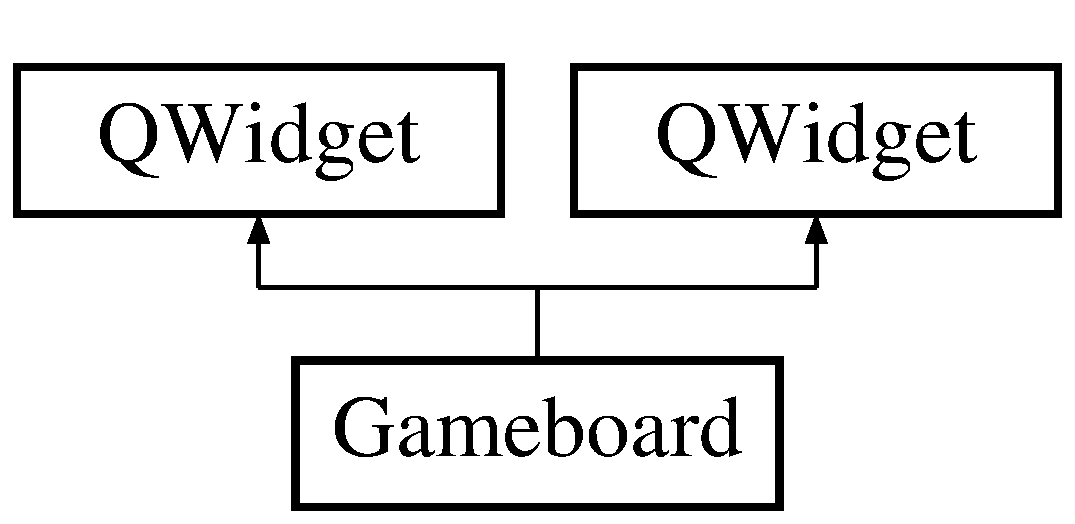
\includegraphics[height=2.000000cm]{class_gameboard}
\end{center}
\end{figure}
\subsection*{Public Slots}
\begin{DoxyCompactItemize}
\item 
\hypertarget{class_gameboard_a1447e62dd9f78bcba4bdb06c4bfb8f10}{}void {\bfseries resume\+Game} ()\label{class_gameboard_a1447e62dd9f78bcba4bdb06c4bfb8f10}

\item 
\hypertarget{class_gameboard_ac59525fc331dafd4a1a290593327aa7c}{}void {\bfseries Slide\+Pingouin} ()\label{class_gameboard_ac59525fc331dafd4a1a290593327aa7c}

\item 
\hypertarget{class_gameboard_aa4e9c04466f50e1590269eab05773581}{}void {\bfseries Slide\+Bloc} ()\label{class_gameboard_aa4e9c04466f50e1590269eab05773581}

\item 
\hypertarget{class_gameboard_af76ebc877764feed7bc9d90452178f5f}{}void {\bfseries exit\+Game} ()\label{class_gameboard_af76ebc877764feed7bc9d90452178f5f}

\item 
\hypertarget{class_gameboard_a0d4ac38611d2ed24732823656ba613e0}{}void {\bfseries restart\+Level} ()\label{class_gameboard_a0d4ac38611d2ed24732823656ba613e0}

\item 
\hypertarget{class_gameboard_a6286269cadea4a1171539b52431d56c5}{}void {\bfseries restart\+Game} ()\label{class_gameboard_a6286269cadea4a1171539b52431d56c5}

\end{DoxyCompactItemize}
\subsection*{Public Member Functions}
\begin{DoxyCompactItemize}
\item 
\hypertarget{class_gameboard_a82157069ecfab2d2245b7d5df563aaae}{}{\bfseries Gameboard} (Q\+Widget $\ast$parent=0)\label{class_gameboard_a82157069ecfab2d2245b7d5df563aaae}

\item 
\hypertarget{class_gameboard_a2ae163b581c0ef4aae6bf1ed0ce7965a}{}Q\+Point $\ast$ {\bfseries get\+Check\+Point} ()\label{class_gameboard_a2ae163b581c0ef4aae6bf1ed0ce7965a}

\end{DoxyCompactItemize}
\subsection*{Static Public Member Functions}
\begin{DoxyCompactItemize}
\item 
\hypertarget{class_gameboard_aa10ed162ff321f4fe480e531ef352bd8}{}static int {\bfseries get\+Game\+Squares} ()\label{class_gameboard_aa10ed162ff321f4fe480e531ef352bd8}

\end{DoxyCompactItemize}
\subsection*{Static Public Attributes}
\begin{DoxyCompactItemize}
\item 
\hypertarget{class_gameboard_a50499cde2f942a0d18d261a7103e1e2a}{}static int {\bfseries size\+X} = 20\label{class_gameboard_a50499cde2f942a0d18d261a7103e1e2a}

\item 
\hypertarget{class_gameboard_a1a60c1746c1bfa669b3bf7b3dfc6534d}{}static int {\bfseries size\+Y} = 15\label{class_gameboard_a1a60c1746c1bfa669b3bf7b3dfc6534d}

\end{DoxyCompactItemize}


The documentation for this class was generated from the following files\+:\begin{DoxyCompactItemize}
\item 
gameboard.\+h\item 
gameboard.\+cpp\end{DoxyCompactItemize}

\hypertarget{class_level}{}\section{Level Class Reference}
\label{class_level}\index{Level@{Level}}
\subsection*{Public Member Functions}
\begin{DoxyCompactItemize}
\item 
\hypertarget{class_level_aba678023dfd388f8ca54dc6a51f8f3e3}{}{\bfseries Level} (int level\+Number)\label{class_level_aba678023dfd388f8ca54dc6a51f8f3e3}

\item 
\hypertarget{class_level_a898937cdec40914b45ecb23649cd5e2a}{}Q\+Graphics\+Scene $\ast$ {\bfseries populate\+Scene} ()\label{class_level_a898937cdec40914b45ecb23649cd5e2a}

\item 
\hypertarget{class_level_ae7176d05829097956f8ba57fcd4155dc}{}Q\+Point $\ast$ {\bfseries get\+Starting\+Point} ()\label{class_level_ae7176d05829097956f8ba57fcd4155dc}

\item 
\hypertarget{class_level_aa1d6d7b228f5b64d697c0cd3666ea836}{}Q\+Point {\bfseries get\+View\+Start} ()\label{class_level_aa1d6d7b228f5b64d697c0cd3666ea836}

\item 
\hypertarget{class_level_adce6f00bfa320883323a9892646cdaa8}{}Q\+Graphics\+Scene $\ast$ {\bfseries change\+Level} (int level\+Number)\label{class_level_adce6f00bfa320883323a9892646cdaa8}

\item 
\hypertarget{class_level_afbf573a6aecae9cba02d7398e5637dd5}{}int {\bfseries get\+Level\+Number} ()\label{class_level_afbf573a6aecae9cba02d7398e5637dd5}

\item 
\hypertarget{class_level_a355ebe125bc8b61b8b7db7543f65bf5e}{}Q\+String {\bfseries get\+Dialog\+Text} ()\label{class_level_a355ebe125bc8b61b8b7db7543f65bf5e}

\end{DoxyCompactItemize}


The documentation for this class was generated from the following files\+:\begin{DoxyCompactItemize}
\item 
level.\+h\item 
level.\+cpp\end{DoxyCompactItemize}

\hypertarget{class_m___pause}{}\section{M\+\_\+\+Pause Class Reference}
\label{class_m___pause}\index{M\+\_\+\+Pause@{M\+\_\+\+Pause}}
Inheritance diagram for M\+\_\+\+Pause\+:\begin{figure}[H]
\begin{center}
\leavevmode
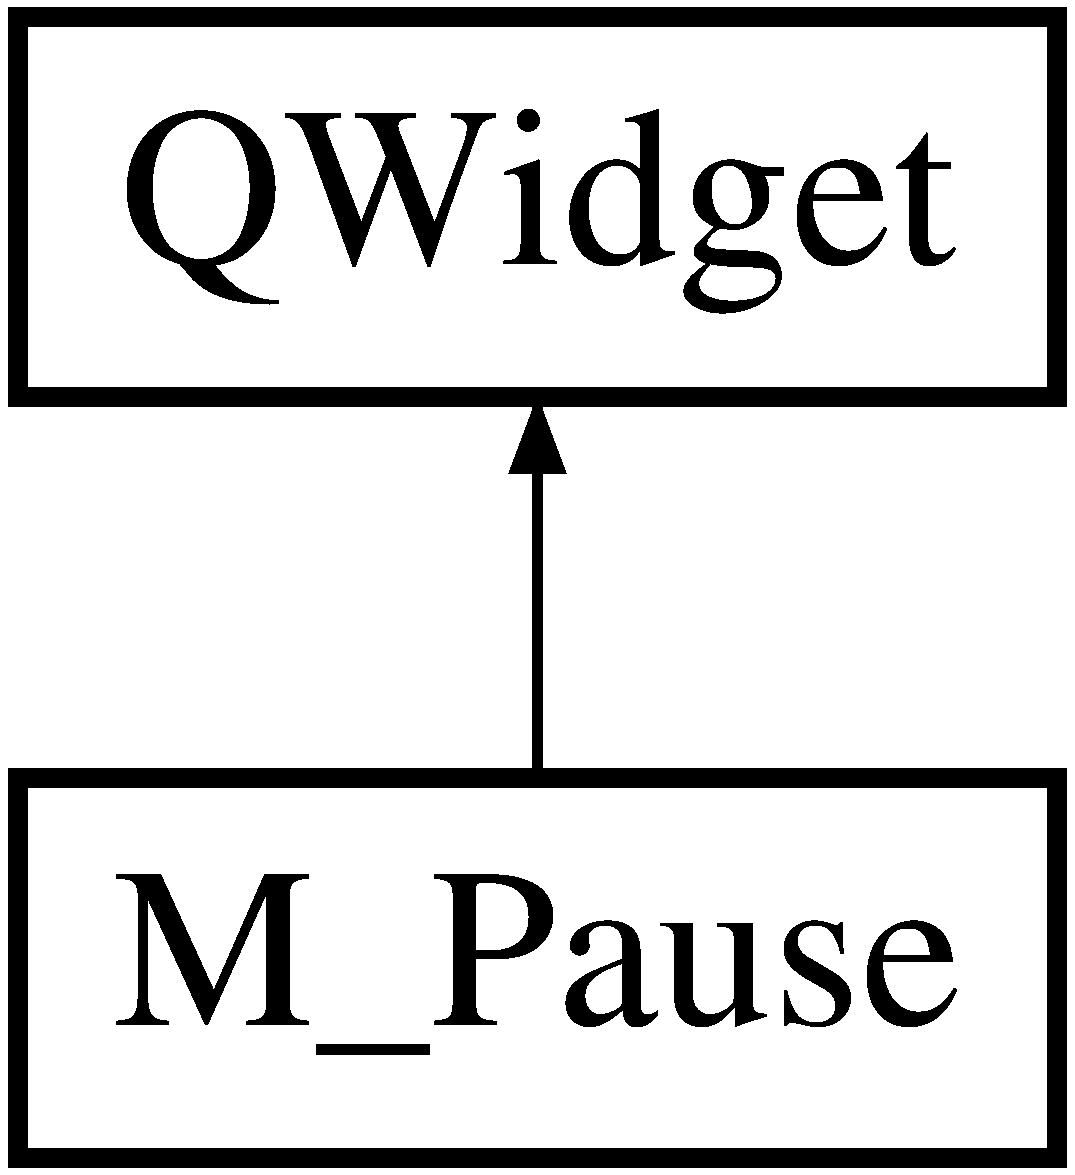
\includegraphics[height=2.000000cm]{class_m___pause}
\end{center}
\end{figure}
\subsection*{Public Member Functions}
\begin{DoxyCompactItemize}
\item 
\hypertarget{class_m___pause_ac1cb95e28d9c158d4dfdba4a08491432}{}{\bfseries M\+\_\+\+Pause} (Q\+Widget $\ast$parent)\label{class_m___pause_ac1cb95e28d9c158d4dfdba4a08491432}

\item 
\hypertarget{class_m___pause_a1c4c4a10f597d250973481b81d575e14}{}void {\bfseries set\+Unable\+Menu} (int level\+Value)\label{class_m___pause_a1c4c4a10f597d250973481b81d575e14}

\end{DoxyCompactItemize}


The documentation for this class was generated from the following files\+:\begin{DoxyCompactItemize}
\item 
m\+\_\+pause.\+h\item 
m\+\_\+pause.\+cpp\end{DoxyCompactItemize}

\hypertarget{class_main_game}{}\section{Main\+Game Class Reference}
\label{class_main_game}\index{Main\+Game@{Main\+Game}}


Managing the backend of the game.  




{\ttfamily \#include $<$maingame.\+h$>$}

Inheritance diagram for Main\+Game\+:\begin{figure}[H]
\begin{center}
\leavevmode
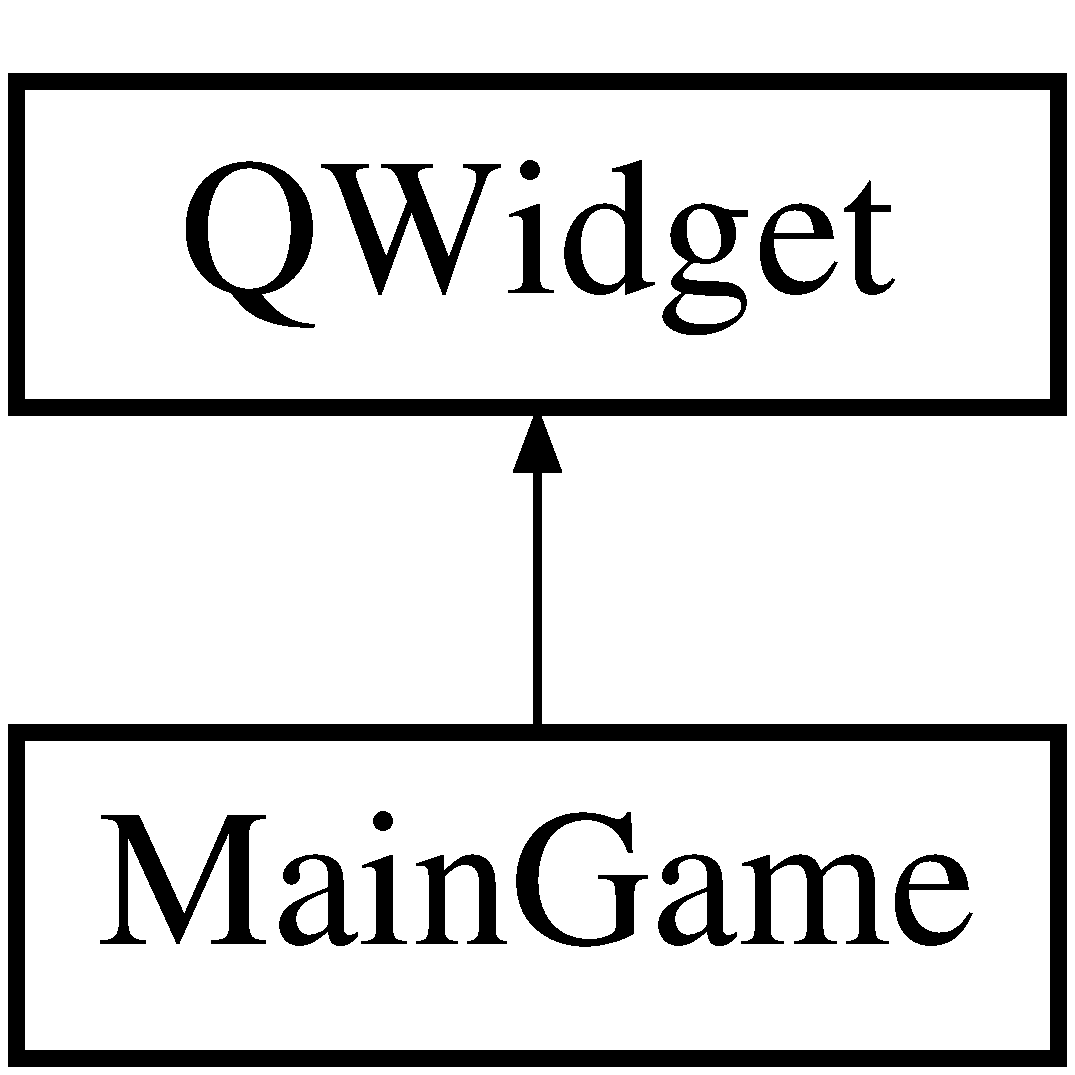
\includegraphics[height=2.000000cm]{class_main_game}
\end{center}
\end{figure}
\subsection*{Public Slots}
\begin{DoxyCompactItemize}
\item 
\hypertarget{class_main_game_aab3b497b7d0de1bcc87175895f477a9c}{}void {\bfseries start\+Game} (\hyperlink{class_profil}{Profil} $\ast$user)\label{class_main_game_aab3b497b7d0de1bcc87175895f477a9c}

\item 
\hypertarget{class_main_game_a21e0447f9ff6eeaa12d8abbd7c34aafe}{}void {\bfseries refresh\+Game\+Menu} ()\label{class_main_game_a21e0447f9ff6eeaa12d8abbd7c34aafe}

\end{DoxyCompactItemize}
\subsection*{Public Member Functions}
\begin{DoxyCompactItemize}
\item 
\hypertarget{class_main_game_aba77e63bf031bc452693ba06986affe6}{}{\bfseries Main\+Game} (Q\+Widget $\ast$parent=0)\label{class_main_game_aba77e63bf031bc452693ba06986affe6}

\end{DoxyCompactItemize}


\subsection{Detailed Description}
Managing the backend of the game. 

It shows the main menu, \hyperlink{class_menu_start}{Menu\+Start}. It does the transition between the \hyperlink{class_menu_start}{Menu\+Start} and the \hyperlink{class_gameboard}{Gameboard}. Gives the graphical structure for the video game and the O\+S on which it\textquotesingle{}s run. \begin{DoxyAuthor}{Author}
Claret Romain, \href{mailto:romain.claret@rocla.ch}{\tt romain.\+claret@rocla.\+ch} 

Divernois Margaux, \href{mailto:margaux.divernois@gmail.com}{\tt margaux.\+divernois@gmail.\+com} 

Visinand Steve, \href{mailto:visinandst@gmail.com}{\tt visinandst@gmail.\+com} 
\end{DoxyAuthor}
\begin{DoxyCopyright}{Copyright}
Custom License + N\+D\+A 
\end{DoxyCopyright}
\begin{DoxyVersion}{Version}
1.\+0 
\end{DoxyVersion}
\begin{DoxyDate}{Date}
27 January 2015 
\end{DoxyDate}
\begin{DoxyRefDesc}{Todo}
\item[\hyperlink{todo__todo000029}{Todo}]Manage the close event correctly, because it\textquotesingle{}s painful when just in the \hyperlink{class_menu_start}{Menu\+Start}. \end{DoxyRefDesc}


The documentation for this class was generated from the following files\+:\begin{DoxyCompactItemize}
\item 
maingame.\+h\item 
maingame.\+cpp\end{DoxyCompactItemize}

\hypertarget{class_menu_start}{}\section{Menu\+Start Class Reference}
\label{class_menu_start}\index{Menu\+Start@{Menu\+Start}}


Main menu, which appears at the game startup.  




{\ttfamily \#include $<$m\+\_\+menustart.\+h$>$}

Inheritance diagram for Menu\+Start\+:\begin{figure}[H]
\begin{center}
\leavevmode
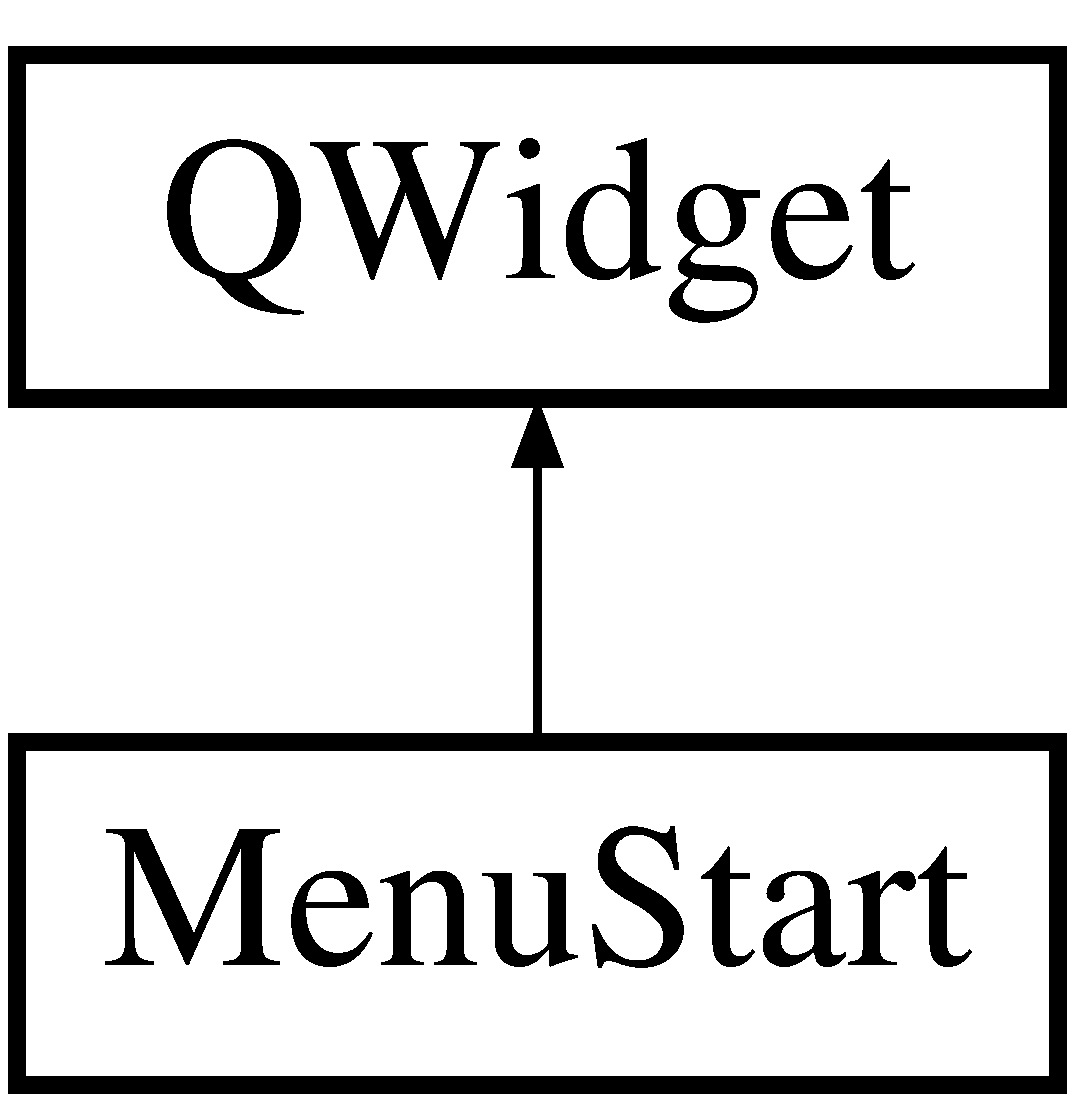
\includegraphics[height=2.000000cm]{class_menu_start}
\end{center}
\end{figure}
\subsection*{Public Slots}
\begin{DoxyCompactItemize}
\item 
\hypertarget{class_menu_start_a8af8ec946e4b575852937b469bfe3d59}{}void {\bfseries load\+Game} (Q\+String value)\label{class_menu_start_a8af8ec946e4b575852937b469bfe3d59}

\item 
\hypertarget{class_menu_start_a3ebce084546f1f9374a2e1cd0378d17a}{}void {\bfseries new\+Game} ()\label{class_menu_start_a3ebce084546f1f9374a2e1cd0378d17a}

\item 
\hypertarget{class_menu_start_a27892e476830d761fae92cc8b7db323f}{}void {\bfseries new\+Game\+Form} ()\label{class_menu_start_a27892e476830d761fae92cc8b7db323f}

\end{DoxyCompactItemize}
\subsection*{Signals}
\begin{DoxyCompactItemize}
\item 
\hypertarget{class_menu_start_a6bb370ac28c64683a712f30b19a97bc8}{}void {\bfseries start\+Game} (\hyperlink{class_profil}{Profil} $\ast$)\label{class_menu_start_a6bb370ac28c64683a712f30b19a97bc8}

\item 
\hypertarget{class_menu_start_a277ad4799e66f6b7e314d159467bc963}{}void {\bfseries refresh\+Game\+Menu} ()\label{class_menu_start_a277ad4799e66f6b7e314d159467bc963}

\end{DoxyCompactItemize}
\subsection*{Public Member Functions}
\begin{DoxyCompactItemize}
\item 
\hypertarget{class_menu_start_a184ff65bb2534378670fee22487b02eb}{}{\bfseries Menu\+Start} (Q\+Widget $\ast$parent=0)\label{class_menu_start_a184ff65bb2534378670fee22487b02eb}

\item 
\hypertarget{class_menu_start_aa472610f5ba9e271cb02159d2ca421cc}{}bool {\bfseries get\+Profil} ()\label{class_menu_start_aa472610f5ba9e271cb02159d2ca421cc}

\end{DoxyCompactItemize}
\subsection*{Static Public Member Functions}
\begin{DoxyCompactItemize}
\item 
\hypertarget{class_menu_start_a7cb6adad5555d8eb90e27bed5e4333c5}{}static void {\bfseries save\+Game} (\hyperlink{class_profil}{Profil} $\ast$current\+User)\label{class_menu_start_a7cb6adad5555d8eb90e27bed5e4333c5}

\end{DoxyCompactItemize}
\subsection*{Public Attributes}
\begin{DoxyCompactItemize}
\item 
\hypertarget{class_menu_start_a04d0eac4832176f91f62172757ce0616}{}Q\+List$<$ Q\+Push\+Button $\ast$ $>$ $\ast$ {\bfseries list\+Button\+Profil}\label{class_menu_start_a04d0eac4832176f91f62172757ce0616}

\item 
\hypertarget{class_menu_start_af01ac293a06b0da924be0ad29aa587cf}{}Q\+Push\+Button $\ast$ {\bfseries button\+New}\label{class_menu_start_af01ac293a06b0da924be0ad29aa587cf}

\item 
\hypertarget{class_menu_start_a9426199e93ab1722b19b4e4e178b0164}{}Q\+V\+Box\+Layout $\ast$ {\bfseries layout\+Menu}\label{class_menu_start_a9426199e93ab1722b19b4e4e178b0164}

\item 
\hypertarget{class_menu_start_abf21ea1841ef22859a15b1c201b8bbf6}{}Q\+Line\+Edit $\ast$ {\bfseries username}\label{class_menu_start_abf21ea1841ef22859a15b1c201b8bbf6}

\item 
\hypertarget{class_menu_start_a06ebe4101b60777e4e1465e1073d533b}{}Q\+Push\+Button $\ast$ {\bfseries validate}\label{class_menu_start_a06ebe4101b60777e4e1465e1073d533b}

\item 
\hypertarget{class_menu_start_a427333babe7349783094bc9257462cb0}{}Q\+Label $\ast$ {\bfseries text\+Pseudo}\label{class_menu_start_a427333babe7349783094bc9257462cb0}

\end{DoxyCompactItemize}


\subsection{Detailed Description}
Main menu, which appears at the game startup. 

It allows the user to select or create a profil and run a game. Games are saved in a json file type. Saves are found in\+: Mac\+O\+S\+X \+: \char`\"{}\+Game.\+app/\+Contents/\+Mac\+O\+S/save.\+json\char`\"{}, Windows \+: Dans le meme dossier que Game.\+exe. Save files are not encrypted. \begin{DoxyAuthor}{Author}
Claret Romain, \href{mailto:romain.claret@rocla.ch}{\tt romain.\+claret@rocla.\+ch} 

Divernois Margaux, \href{mailto:margaux.divernois@gmail.com}{\tt margaux.\+divernois@gmail.\+com} 

Visinand Steve, \href{mailto:visinandst@gmail.com}{\tt visinandst@gmail.\+com} 
\end{DoxyAuthor}
\begin{DoxyCopyright}{Copyright}
Custom License + N\+D\+A 
\end{DoxyCopyright}
\begin{DoxyVersion}{Version}
1.\+0 
\end{DoxyVersion}
\begin{DoxyDate}{Date}
27 January 2015 
\end{DoxyDate}
\begin{DoxyRefDesc}{Todo}
\item[\hyperlink{todo__todo000013}{Todo}]encrypt save files 

add credits \end{DoxyRefDesc}


The documentation for this class was generated from the following files\+:\begin{DoxyCompactItemize}
\item 
m\+\_\+menustart.\+h\item 
m\+\_\+menustart.\+cpp\end{DoxyCompactItemize}

\hypertarget{class_object}{}\section{Object Class Reference}
\label{class_object}\index{Object@{Object}}


\hyperlink{class_object}{Object} from the game.  




{\ttfamily \#include $<$object.\+h$>$}

Inheritance diagram for Object\+:\begin{figure}[H]
\begin{center}
\leavevmode
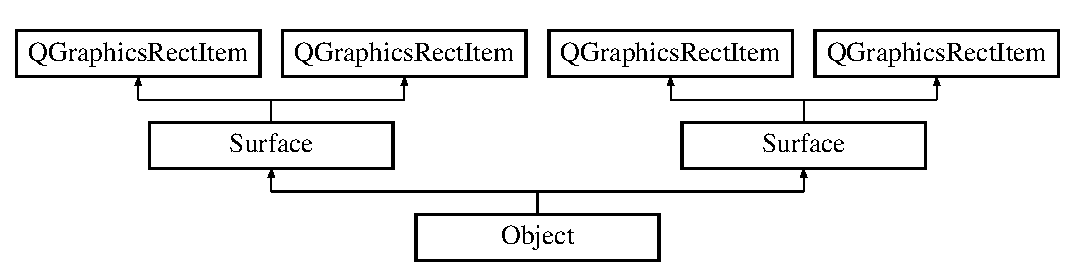
\includegraphics[height=3.000000cm]{class_object}
\end{center}
\end{figure}
\subsection*{Public Member Functions}
\begin{DoxyCompactItemize}
\item 
\hypertarget{class_object_a61b5e9862ead7000e3125be5d81263a2}{}{\bfseries Object} (int xpos, int ypos, Q\+Graphics\+Item $\ast$parent)\label{class_object_a61b5e9862ead7000e3125be5d81263a2}

\item 
\hypertarget{class_object_a92bae89e044afc5957483772f557c5d7}{}{\bfseries Object} (Q\+String new\+\_\+nom, Q\+Graphics\+Item $\ast$parent=0)\label{class_object_a92bae89e044afc5957483772f557c5d7}

\item 
\hypertarget{class_object_a64d92ae18b1e70a8435690fe6fccf1fd}{}void {\bfseries set\+Design} ()\label{class_object_a64d92ae18b1e70a8435690fe6fccf1fd}

\item 
\hypertarget{class_object_a13fe059222e66ea54aa3f6f8615a3d72}{}Q\+String {\bfseries get\+Name} ()\label{class_object_a13fe059222e66ea54aa3f6f8615a3d72}

\item 
\hypertarget{class_object_a2678fa7a8ab432607b228e8d311f2873}{}Q\+Pixmap {\bfseries get\+Texture} ()\label{class_object_a2678fa7a8ab432607b228e8d311f2873}

\end{DoxyCompactItemize}


\subsection{Detailed Description}
\hyperlink{class_object}{Object} from the game. 

Set the object\textquotesingle{}s info and its skin. \begin{DoxyAuthor}{Author}
Claret Romain, \href{mailto:romain.claret@rocla.ch}{\tt romain.\+claret@rocla.\+ch} 

Divernois Margaux, \href{mailto:margaux.divernois@gmail.com}{\tt margaux.\+divernois@gmail.\+com} 

Visinand Steve, \href{mailto:visinandst@gmail.com}{\tt visinandst@gmail.\+com} 
\end{DoxyAuthor}
\begin{DoxyCopyright}{Copyright}
Custom License + N\+D\+A 
\end{DoxyCopyright}
\begin{DoxyVersion}{Version}
1.\+0 
\end{DoxyVersion}
\begin{DoxyDate}{Date}
27 January 2015 
\end{DoxyDate}


The documentation for this class was generated from the following files\+:\begin{DoxyCompactItemize}
\item 
object.\+h\item 
object.\+cpp\end{DoxyCompactItemize}

\hypertarget{class_pingouin}{}\section{Pingouin Class Reference}
\label{class_pingouin}\index{Pingouin@{Pingouin}}
Inheritance diagram for Pingouin\+:\begin{figure}[H]
\begin{center}
\leavevmode
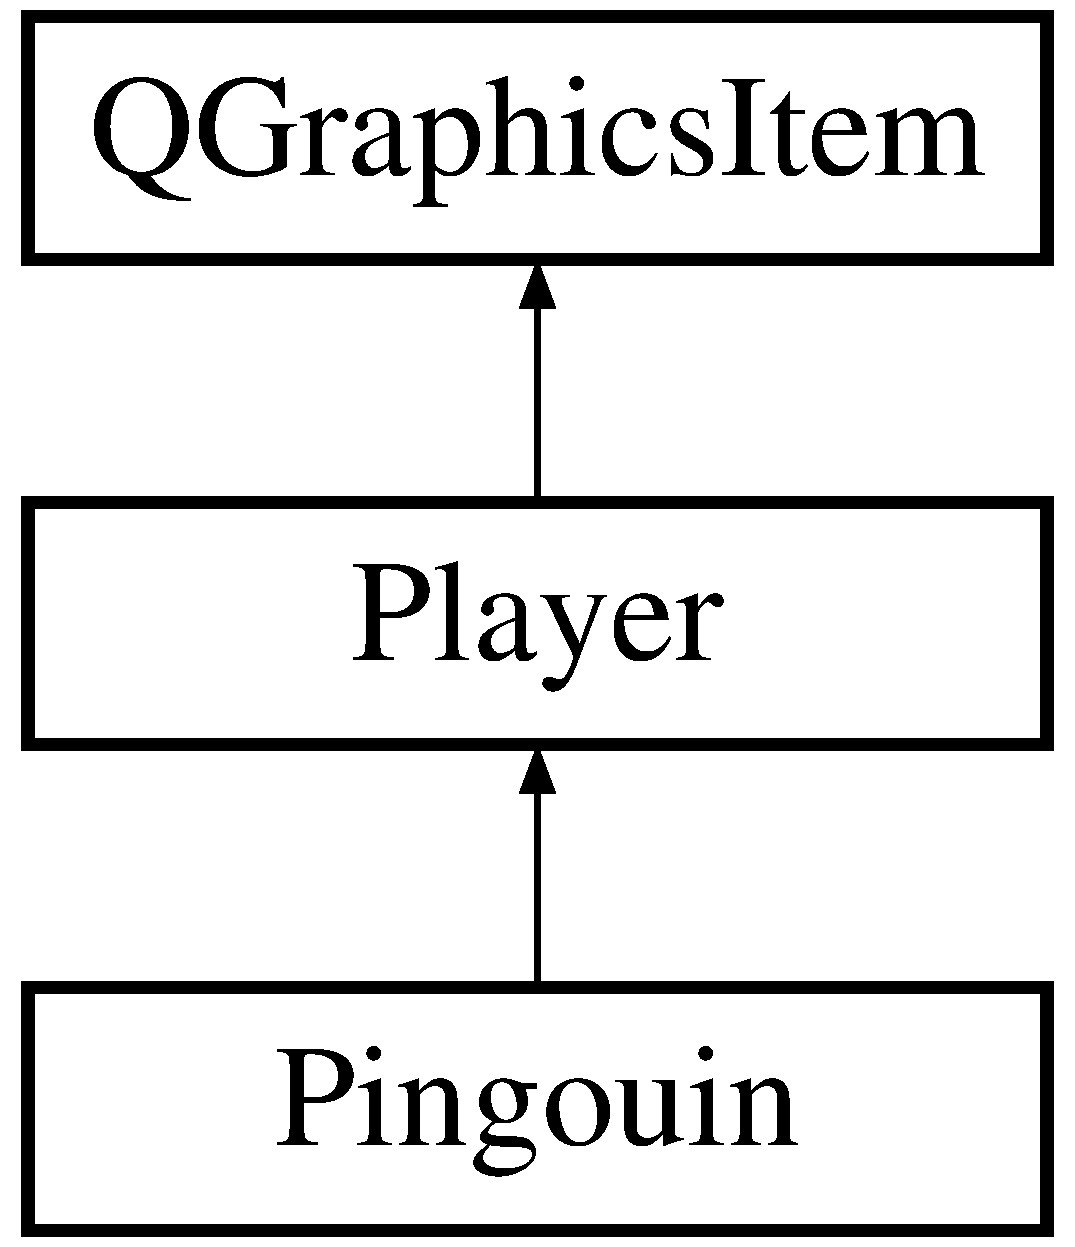
\includegraphics[height=3.000000cm]{class_pingouin}
\end{center}
\end{figure}
\subsection*{Public Member Functions}
\begin{DoxyCompactItemize}
\item 
\hypertarget{class_pingouin_a91f0120d2ee61c6a6ca715a8e88f3d3b}{}void {\bfseries set\+Pos} (int, int)\label{class_pingouin_a91f0120d2ee61c6a6ca715a8e88f3d3b}

\item 
\hypertarget{class_pingouin_a80aa8b486de1bba6c637a8ab0233fc10}{}void {\bfseries move\+By} (int, int)\label{class_pingouin_a80aa8b486de1bba6c637a8ab0233fc10}

\item 
\hypertarget{class_pingouin_a6b74f3acac4cce611992586356805d4a}{}void {\bfseries move\+Back} ()\label{class_pingouin_a6b74f3acac4cce611992586356805d4a}

\item 
\hypertarget{class_pingouin_a90eef5bc5b47bdae1508f572d1d898d5}{}void {\bfseries add\+To\+Scene} (Q\+Graphics\+Scene $\ast$)\label{class_pingouin_a90eef5bc5b47bdae1508f572d1d898d5}

\item 
\hypertarget{class_pingouin_ad91b21a996f75e32a78c203eb7490446}{}void {\bfseries add\+Object\+To\+Sacoche} (\hyperlink{class_object}{Object} $\ast$object)\label{class_pingouin_ad91b21a996f75e32a78c203eb7490446}

\item 
\hypertarget{class_pingouin_a73130bc706f0c1a40a20f05d0d3a3ffa}{}void {\bfseries remove\+Object\+From\+Sacoche} (Q\+String object)\label{class_pingouin_a73130bc706f0c1a40a20f05d0d3a3ffa}

\item 
\hypertarget{class_pingouin_a7bc2b0b92b4093f59821a683e6d71b14}{}void {\bfseries remove\+Temp\+From\+Sacoche} ()\label{class_pingouin_a7bc2b0b92b4093f59821a683e6d71b14}

\item 
\hypertarget{class_pingouin_a53145c212327b2a733237e1eb55aad24}{}bool {\bfseries check\+Object\+Sacoche} (Q\+String object, int quantity=1)\label{class_pingouin_a53145c212327b2a733237e1eb55aad24}

\item 
\hypertarget{class_pingouin_aa5ed410fe91fcdf598b00baf4c33354f}{}Q\+List$<$ \hyperlink{class_object}{Object} $\ast$ $>$ {\bfseries get\+Sacoche} ()\label{class_pingouin_aa5ed410fe91fcdf598b00baf4c33354f}

\item 
\hypertarget{class_pingouin_a736f73e55524b59c00479aef1f91f94d}{}void {\bfseries print\+Sacoche} ()\label{class_pingouin_a736f73e55524b59c00479aef1f91f94d}

\item 
\hypertarget{class_pingouin_a1adb59f85236324915f9211bc111faa6}{}void {\bfseries empty\+Temp\+Sacoche} ()\label{class_pingouin_a1adb59f85236324915f9211bc111faa6}

\item 
\hypertarget{class_pingouin_af53b1d8d5167cd2fc039f97219f22064}{}void {\bfseries empty\+Sacoche} ()\label{class_pingouin_af53b1d8d5167cd2fc039f97219f22064}

\item 
\hypertarget{class_pingouin_a31dcd728180d2e85cf1c696ad2f0b062}{}bool {\bfseries is\+Slide} ()\label{class_pingouin_a31dcd728180d2e85cf1c696ad2f0b062}

\item 
\hypertarget{class_pingouin_aecce86d070fcfef325a55676043866ab}{}void {\bfseries set\+Slide\+Able} (bool value)\label{class_pingouin_aecce86d070fcfef325a55676043866ab}

\item 
\hypertarget{class_pingouin_ad571ffa2df0cdb3a6381bd24ec1363eb}{}Q\+Graphics\+Rect\+Item $\ast$ {\bfseries get\+Collide\+Bloc} (char sens\+Depl)\label{class_pingouin_ad571ffa2df0cdb3a6381bd24ec1363eb}

\item 
\hypertarget{class_pingouin_ab65df246ceda4f50ec939faeb55a9550}{}Q\+List$<$ Q\+Graphics\+Item $\ast$ $>$ {\bfseries Collides\+Right} ()\label{class_pingouin_ab65df246ceda4f50ec939faeb55a9550}

\item 
\hypertarget{class_pingouin_a4775b4894d8b8165c778019de8df2d15}{}Q\+List$<$ Q\+Graphics\+Item $\ast$ $>$ {\bfseries Collides\+Left} ()\label{class_pingouin_a4775b4894d8b8165c778019de8df2d15}

\item 
\hypertarget{class_pingouin_aa81d4eaddce1ef53808d6d4978d1b132}{}Q\+List$<$ Q\+Graphics\+Item $\ast$ $>$ {\bfseries Collides\+Top} ()\label{class_pingouin_aa81d4eaddce1ef53808d6d4978d1b132}

\item 
\hypertarget{class_pingouin_af7dbd1097ef3d4cf4911d006fa67f06e}{}Q\+List$<$ Q\+Graphics\+Item $\ast$ $>$ {\bfseries Collides\+Bottom} ()\label{class_pingouin_af7dbd1097ef3d4cf4911d006fa67f06e}

\item 
\hypertarget{class_pingouin_a10126ab2598c56da1fe96bae1bedf9a7}{}Q\+List$<$ Q\+Graphics\+Item $\ast$ $>$ {\bfseries Collides\+Center} ()\label{class_pingouin_a10126ab2598c56da1fe96bae1bedf9a7}

\item 
\hypertarget{class_pingouin_aaa130c988fb99be84ae8ce057ff0466f}{}Q\+Graphics\+Rect\+Item $\ast$ {\bfseries get\+Left\+C\+B} ()\label{class_pingouin_aaa130c988fb99be84ae8ce057ff0466f}

\item 
\hypertarget{class_pingouin_a840603a098f62619f3cf6aef3ff71500}{}Q\+Graphics\+Rect\+Item $\ast$ {\bfseries get\+Right\+C\+B} ()\label{class_pingouin_a840603a098f62619f3cf6aef3ff71500}

\item 
\hypertarget{class_pingouin_a04bb88b6251aa853e1980c35005f7df8}{}Q\+Graphics\+Rect\+Item $\ast$ {\bfseries get\+Top\+C\+B} ()\label{class_pingouin_a04bb88b6251aa853e1980c35005f7df8}

\item 
\hypertarget{class_pingouin_aafa634e4ec962a442b5a4fdf1d029464}{}Q\+Graphics\+Rect\+Item $\ast$ {\bfseries get\+Bottom\+C\+B} ()\label{class_pingouin_aafa634e4ec962a442b5a4fdf1d029464}

\item 
\hypertarget{class_pingouin_ae8bf1799a91f7c7863731ddcfe1b1418}{}\hyperlink{class_player}{Player} $\ast$ {\bfseries get\+Player} ()\label{class_pingouin_ae8bf1799a91f7c7863731ddcfe1b1418}

\end{DoxyCompactItemize}
\subsection*{Additional Inherited Members}


The documentation for this class was generated from the following files\+:\begin{DoxyCompactItemize}
\item 
p\+\_\+penguin.\+h\item 
p\+\_\+penguin.\+cpp\end{DoxyCompactItemize}

\hypertarget{class_player}{}\section{Player Class Reference}
\label{class_player}\index{Player@{Player}}
Inheritance diagram for Player\+:\begin{figure}[H]
\begin{center}
\leavevmode
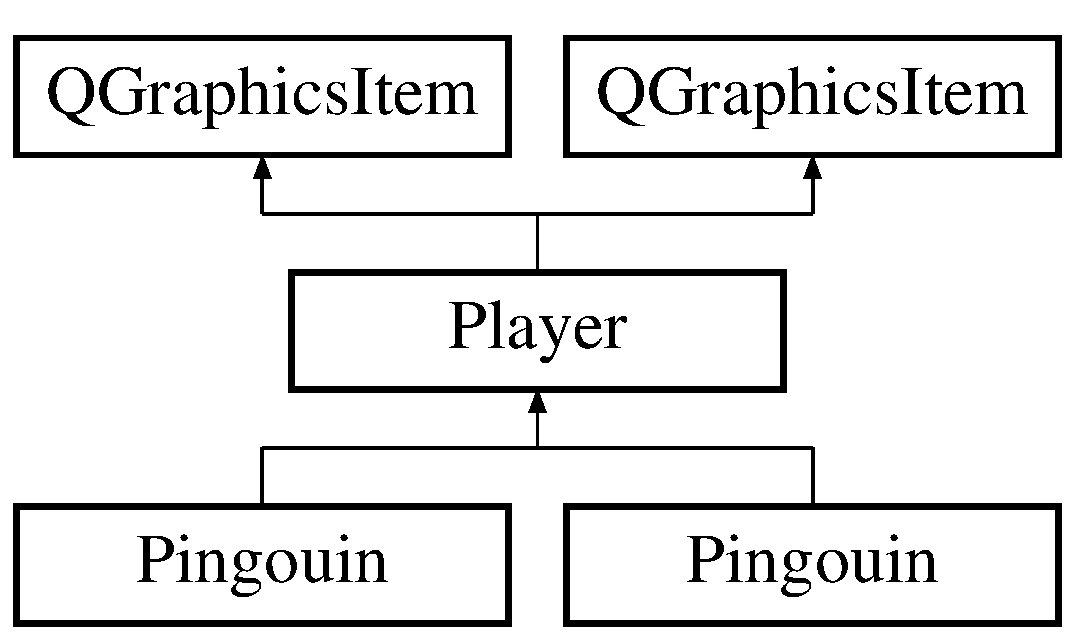
\includegraphics[height=3.000000cm]{class_player}
\end{center}
\end{figure}
\subsection*{Public Member Functions}
\begin{DoxyCompactItemize}
\item 
\hypertarget{class_player_a40e85189b099c86221a8ad62f3173980}{}Q\+Rect\+F {\bfseries bounding\+Rect} () const \label{class_player_a40e85189b099c86221a8ad62f3173980}

\item 
\hypertarget{class_player_a02d1d7a8488bc2ed3a9b317dcf17b39c}{}void {\bfseries paint} (Q\+Painter $\ast$painter, const Q\+Style\+Option\+Graphics\+Item $\ast$option, Q\+Widget $\ast$widget)\label{class_player_a02d1d7a8488bc2ed3a9b317dcf17b39c}

\item 
\hypertarget{class_player_a80ee830f8960d206559305a257e34dcb}{}void {\bfseries set\+Player\+Orientation} (Q\+String orientation)\label{class_player_a80ee830f8960d206559305a257e34dcb}

\item 
\hypertarget{class_player_a7c71ec72ae01aa19ffff508fe61df393}{}Q\+String {\bfseries get\+Player\+Orientation} ()\label{class_player_a7c71ec72ae01aa19ffff508fe61df393}

\item 
\hypertarget{class_player_aab3077d4bd36a08a88a618b56a115b1e}{}Q\+Point $\ast$ {\bfseries get\+Pos} ()\label{class_player_aab3077d4bd36a08a88a618b56a115b1e}

\end{DoxyCompactItemize}
\subsection*{Public Attributes}
\begin{DoxyCompactItemize}
\item 
\hypertarget{class_player_aa6bebd35f8a777820886664b9444b9b5}{}Q\+Brush $\ast$ {\bfseries player\+Skin}\label{class_player_aa6bebd35f8a777820886664b9444b9b5}

\end{DoxyCompactItemize}
\subsection*{Protected Attributes}
\begin{DoxyCompactItemize}
\item 
\hypertarget{class_player_aa3c4b095965da25dba3e777122082773}{}int {\bfseries x\+Pos}\label{class_player_aa3c4b095965da25dba3e777122082773}

\item 
\hypertarget{class_player_a0a14d018fcc4b1ad121dce82524d3c96}{}int {\bfseries y\+Pos}\label{class_player_a0a14d018fcc4b1ad121dce82524d3c96}

\end{DoxyCompactItemize}


The documentation for this class was generated from the following files\+:\begin{DoxyCompactItemize}
\item 
player.\+h\item 
player.\+cpp\end{DoxyCompactItemize}

\hypertarget{class_profil}{}\section{Profil Class Reference}
\label{class_profil}\index{Profil@{Profil}}


\hyperlink{class_player}{Player}\textquotesingle{}s profil management.  




{\ttfamily \#include $<$profil.\+h$>$}

\subsection*{Public Member Functions}
\begin{DoxyCompactItemize}
\item 
\hypertarget{class_profil_ad874b5e5885c947739f7dfa8a8932442}{}{\bfseries Profil} (const Q\+String \&username)\label{class_profil_ad874b5e5885c947739f7dfa8a8932442}

\item 
\hypertarget{class_profil_af0ab359fbf8feb7e703293c9025e8d36}{}Q\+String {\bfseries get\+Username} ()\label{class_profil_af0ab359fbf8feb7e703293c9025e8d36}

\item 
\hypertarget{class_profil_aa51ac79c413e575f32166eac7694c313}{}Q\+String {\bfseries get\+Start\+Date} ()\label{class_profil_aa51ac79c413e575f32166eac7694c313}

\item 
\hypertarget{class_profil_a9858f08dfaff3155450e2f2a66ae50cf}{}Q\+String {\bfseries get\+Save\+Date} ()\label{class_profil_a9858f08dfaff3155450e2f2a66ae50cf}

\item 
\hypertarget{class_profil_a8c75d1768cb705d48d8d1f0519512e55}{}Q\+String {\bfseries get\+Game\+Time} ()\label{class_profil_a8c75d1768cb705d48d8d1f0519512e55}

\item 
\hypertarget{class_profil_a9755d065b6f920862fdf642af15c7a7d}{}Q\+String {\bfseries get\+Load\+Date} ()\label{class_profil_a9755d065b6f920862fdf642af15c7a7d}

\item 
\hypertarget{class_profil_a5fd30de19283f6ae22a7232dd22e2afa}{}int {\bfseries get\+Level} ()\label{class_profil_a5fd30de19283f6ae22a7232dd22e2afa}

\item 
\hypertarget{class_profil_aea2c7ddbba5567c777b37293f5fa2aaa}{}Q\+List$<$ int $>$ {\bfseries get\+Power} ()\label{class_profil_aea2c7ddbba5567c777b37293f5fa2aaa}

\item 
\hypertarget{class_profil_a4747a4a9cf7d22203bc316f3a0753033}{}int {\bfseries get\+Nb\+Live} ()\label{class_profil_a4747a4a9cf7d22203bc316f3a0753033}

\item 
\hypertarget{class_profil_a10c2f4863000e5525f8504a22ccf1260}{}int {\bfseries get\+Difficulty} ()\label{class_profil_a10c2f4863000e5525f8504a22ccf1260}

\item 
\hypertarget{class_profil_a23d36025cd3b9ad9ff128021b16c2431}{}void {\bfseries set\+Username} (Q\+String)\label{class_profil_a23d36025cd3b9ad9ff128021b16c2431}

\item 
\hypertarget{class_profil_a3d6b5ead3c4e6af1aa3f4035fb3dd624}{}void {\bfseries set\+Start\+Date} (Q\+String)\label{class_profil_a3d6b5ead3c4e6af1aa3f4035fb3dd624}

\item 
\hypertarget{class_profil_a484838bb61b18b3c82fede9aaad41b35}{}void {\bfseries set\+Save\+Date} (Q\+String)\label{class_profil_a484838bb61b18b3c82fede9aaad41b35}

\item 
\hypertarget{class_profil_a2c9a526c1a26cb8b91c20a3a6df0ccc6}{}void {\bfseries set\+Game\+Time} (Q\+String)\label{class_profil_a2c9a526c1a26cb8b91c20a3a6df0ccc6}

\item 
\hypertarget{class_profil_a7edbce434f4b1c1bf1d98b704fcc650e}{}void {\bfseries set\+Level} (int)\label{class_profil_a7edbce434f4b1c1bf1d98b704fcc650e}

\item 
\hypertarget{class_profil_a1322566ebccffe1636df61c9bc74695d}{}void {\bfseries set\+Power} (Q\+List$<$ int $>$)\label{class_profil_a1322566ebccffe1636df61c9bc74695d}

\item 
\hypertarget{class_profil_ae8d5b07cd8bd4d8ad2a1e1b431056a0f}{}void {\bfseries set\+Nb\+Live} (int)\label{class_profil_ae8d5b07cd8bd4d8ad2a1e1b431056a0f}

\item 
\hypertarget{class_profil_ab4c02fb71667985e9e9ffe991ea6b824}{}void {\bfseries set\+Difficulty} (int)\label{class_profil_ab4c02fb71667985e9e9ffe991ea6b824}

\item 
\hypertarget{class_profil_ab834326ebb9864fca5aec8020d0ad6f8}{}void {\bfseries read} (const Q\+Json\+Object \&json)\label{class_profil_ab834326ebb9864fca5aec8020d0ad6f8}

\item 
\hypertarget{class_profil_a0c07c8aaf3e8b1fee2aeb5ee226f4206}{}void {\bfseries write} (Q\+Json\+Object \&json) const \label{class_profil_a0c07c8aaf3e8b1fee2aeb5ee226f4206}

\item 
\hypertarget{class_profil_a6c2dd8fc5f5604ce12959982309eed42}{}void {\bfseries print} ()\label{class_profil_a6c2dd8fc5f5604ce12959982309eed42}

\end{DoxyCompactItemize}
\subsection*{Static Public Attributes}
\begin{DoxyCompactItemize}
\item 
\hypertarget{class_profil_a0b2e757f8408a36260136e1e2033557e}{}static int {\bfseries N\+B\+M\+A\+X\+V\+I\+E} = 99\label{class_profil_a0b2e757f8408a36260136e1e2033557e}

\end{DoxyCompactItemize}


\subsection{Detailed Description}
\hyperlink{class_player}{Player}\textquotesingle{}s profil management. 

Read and write a json file for the profils, which are the saves for the game. It saves player\textquotesingle{}s information and its game advancement and stats. \begin{DoxyAuthor}{Author}
Claret Romain, \href{mailto:romain.claret@rocla.ch}{\tt romain.\+claret@rocla.\+ch} 

Divernois Margaux, \href{mailto:margaux.divernois@gmail.com}{\tt margaux.\+divernois@gmail.\+com} 

Visinand Steve, \href{mailto:visinandst@gmail.com}{\tt visinandst@gmail.\+com} 
\end{DoxyAuthor}
\begin{DoxyCopyright}{Copyright}
Custom License + N\+D\+A 
\end{DoxyCopyright}
\begin{DoxyVersion}{Version}
1.\+0 
\end{DoxyVersion}
\begin{DoxyDate}{Date}
27 January 2015 
\end{DoxyDate}


The documentation for this class was generated from the following files\+:\begin{DoxyCompactItemize}
\item 
profil.\+h\item 
profil.\+cpp\end{DoxyCompactItemize}

\hypertarget{class_s___dialog}{}\section{S\+\_\+\+Dialog Class Reference}
\label{class_s___dialog}\index{S\+\_\+\+Dialog@{S\+\_\+\+Dialog}}


Dialog blocks.  




{\ttfamily \#include $<$s\+\_\+dialog.\+h$>$}

Inheritance diagram for S\+\_\+\+Dialog\+:\begin{figure}[H]
\begin{center}
\leavevmode
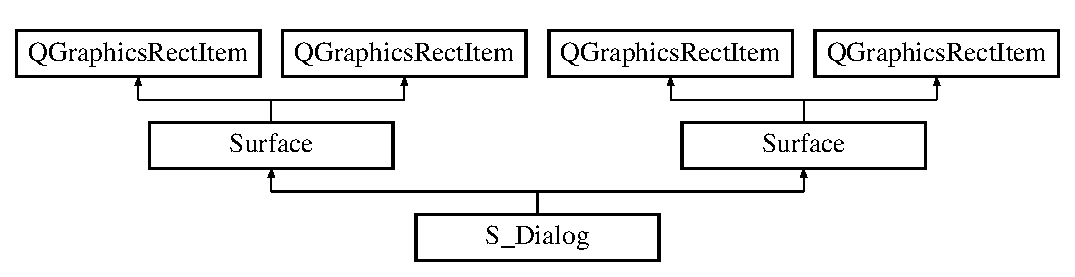
\includegraphics[height=3.000000cm]{class_s___dialog}
\end{center}
\end{figure}
\subsection*{Public Member Functions}
\begin{DoxyCompactItemize}
\item 
\hyperlink{class_s___dialog_a9b20a59ab0954ef8d9befdfbb556e398}{S\+\_\+\+Dialog} (int xpos, int ypos, Q\+Graphics\+Item $\ast$parent=0)
\begin{DoxyCompactList}\small\item\em Constructor with position setup. \end{DoxyCompactList}\item 
\hyperlink{class_s___dialog_a1694750fe7501bc3cd20eb97e1e3384f}{S\+\_\+\+Dialog} (Q\+Graphics\+Item $\ast$parent=0)
\begin{DoxyCompactList}\small\item\em Constructor without position setup. \end{DoxyCompactList}\item 
void \hyperlink{class_s___dialog_a139b0eb3a98042192ac78df37806f1ad}{set\+Dialog\+Number} (int value)
\begin{DoxyCompactList}\small\item\em Set the number of the dialog. \end{DoxyCompactList}\item 
int \hyperlink{class_s___dialog_ad26a628ae1d62d07e1b226126b04814f}{get\+Dialog\+Number} ()
\begin{DoxyCompactList}\small\item\em Get the number of the dialog of self. \end{DoxyCompactList}\item 
void \hyperlink{class_s___dialog_ac156dc3bb16b5c84bce3c710dae215f7}{add\+Dialog\+Text} (Q\+String text)
\begin{DoxyCompactList}\small\item\em Set the dialog of self. \end{DoxyCompactList}\item 
Q\+String \hyperlink{class_s___dialog_aac6c0556054892ff474f485b962027fd}{get\+Text} ()
\begin{DoxyCompactList}\small\item\em Get the dialog of self. \end{DoxyCompactList}\end{DoxyCompactItemize}


\subsection{Detailed Description}
Dialog blocks. 

Surface with a dialog to interact with the player. \begin{DoxyAuthor}{Author}
Claret Romain, \href{mailto:romain.claret@rocla.ch}{\tt romain.\+claret@rocla.\+ch} 

Divernois Margaux, \href{mailto:margaux.divernois@gmail.com}{\tt margaux.\+divernois@gmail.\+com} 

Visinand Steve, \href{mailto:visinandst@gmail.com}{\tt visinandst@gmail.\+com} 
\end{DoxyAuthor}
\begin{DoxyCopyright}{Copyright}
Custom License + N\+D\+A 
\end{DoxyCopyright}
\begin{DoxyVersion}{Version}
1.\+0 
\end{DoxyVersion}
\begin{DoxyDate}{Date}
27 January 2015 
\end{DoxyDate}


\subsection{Constructor \& Destructor Documentation}
\hypertarget{class_s___dialog_a9b20a59ab0954ef8d9befdfbb556e398}{}\index{S\+\_\+\+Dialog@{S\+\_\+\+Dialog}!S\+\_\+\+Dialog@{S\+\_\+\+Dialog}}
\index{S\+\_\+\+Dialog@{S\+\_\+\+Dialog}!S\+\_\+\+Dialog@{S\+\_\+\+Dialog}}
\subsubsection[{S\+\_\+\+Dialog}]{\setlength{\rightskip}{0pt plus 5cm}S\+\_\+\+Dialog\+::\+S\+\_\+\+Dialog (
\begin{DoxyParamCaption}
\item[{int}]{xpos, }
\item[{int}]{ypos, }
\item[{Q\+Graphics\+Item $\ast$}]{parent = {\ttfamily 0}}
\end{DoxyParamCaption}
)}\label{class_s___dialog_a9b20a59ab0954ef8d9befdfbb556e398}


Constructor with position setup. 


\begin{DoxyParams}{Parameters}
{\em xpos} & set the postion on the x-\/axis \\
\hline
{\em ypos} & set the postion on the y-\/axis \\
\hline
{\em parent} & Q\+Graphics\+Item parent \\
\hline
\end{DoxyParams}
\hypertarget{class_s___dialog_a1694750fe7501bc3cd20eb97e1e3384f}{}\index{S\+\_\+\+Dialog@{S\+\_\+\+Dialog}!S\+\_\+\+Dialog@{S\+\_\+\+Dialog}}
\index{S\+\_\+\+Dialog@{S\+\_\+\+Dialog}!S\+\_\+\+Dialog@{S\+\_\+\+Dialog}}
\subsubsection[{S\+\_\+\+Dialog}]{\setlength{\rightskip}{0pt plus 5cm}S\+\_\+\+Dialog\+::\+S\+\_\+\+Dialog (
\begin{DoxyParamCaption}
\item[{Q\+Graphics\+Item $\ast$}]{parent = {\ttfamily 0}}
\end{DoxyParamCaption}
)}\label{class_s___dialog_a1694750fe7501bc3cd20eb97e1e3384f}


Constructor without position setup. 


\begin{DoxyParams}{Parameters}
{\em parent} & Q\+Graphics\+Item to depend on \\
\hline
\end{DoxyParams}


\subsection{Member Function Documentation}
\hypertarget{class_s___dialog_ac156dc3bb16b5c84bce3c710dae215f7}{}\index{S\+\_\+\+Dialog@{S\+\_\+\+Dialog}!add\+Dialog\+Text@{add\+Dialog\+Text}}
\index{add\+Dialog\+Text@{add\+Dialog\+Text}!S\+\_\+\+Dialog@{S\+\_\+\+Dialog}}
\subsubsection[{add\+Dialog\+Text}]{\setlength{\rightskip}{0pt plus 5cm}void S\+\_\+\+Dialog\+::add\+Dialog\+Text (
\begin{DoxyParamCaption}
\item[{Q\+String}]{text}
\end{DoxyParamCaption}
)}\label{class_s___dialog_ac156dc3bb16b5c84bce3c710dae215f7}


Set the dialog of self. 


\begin{DoxyParams}{Parameters}
{\em text} & \\
\hline
\end{DoxyParams}
\hypertarget{class_s___dialog_ad26a628ae1d62d07e1b226126b04814f}{}\index{S\+\_\+\+Dialog@{S\+\_\+\+Dialog}!get\+Dialog\+Number@{get\+Dialog\+Number}}
\index{get\+Dialog\+Number@{get\+Dialog\+Number}!S\+\_\+\+Dialog@{S\+\_\+\+Dialog}}
\subsubsection[{get\+Dialog\+Number}]{\setlength{\rightskip}{0pt plus 5cm}int S\+\_\+\+Dialog\+::get\+Dialog\+Number (
\begin{DoxyParamCaption}
{}
\end{DoxyParamCaption}
)}\label{class_s___dialog_ad26a628ae1d62d07e1b226126b04814f}


Get the number of the dialog of self. 


\begin{DoxyParams}{Parameters}
{\em value} & \\
\hline
\end{DoxyParams}
\hypertarget{class_s___dialog_aac6c0556054892ff474f485b962027fd}{}\index{S\+\_\+\+Dialog@{S\+\_\+\+Dialog}!get\+Text@{get\+Text}}
\index{get\+Text@{get\+Text}!S\+\_\+\+Dialog@{S\+\_\+\+Dialog}}
\subsubsection[{get\+Text}]{\setlength{\rightskip}{0pt plus 5cm}Q\+String S\+\_\+\+Dialog\+::get\+Text (
\begin{DoxyParamCaption}
{}
\end{DoxyParamCaption}
)}\label{class_s___dialog_aac6c0556054892ff474f485b962027fd}


Get the dialog of self. 

\begin{DoxyReturn}{Returns}
text of the dialog 
\end{DoxyReturn}
\hypertarget{class_s___dialog_a139b0eb3a98042192ac78df37806f1ad}{}\index{S\+\_\+\+Dialog@{S\+\_\+\+Dialog}!set\+Dialog\+Number@{set\+Dialog\+Number}}
\index{set\+Dialog\+Number@{set\+Dialog\+Number}!S\+\_\+\+Dialog@{S\+\_\+\+Dialog}}
\subsubsection[{set\+Dialog\+Number}]{\setlength{\rightskip}{0pt plus 5cm}void S\+\_\+\+Dialog\+::set\+Dialog\+Number (
\begin{DoxyParamCaption}
\item[{int}]{value}
\end{DoxyParamCaption}
)}\label{class_s___dialog_a139b0eb3a98042192ac78df37806f1ad}


Set the number of the dialog. 


\begin{DoxyParams}{Parameters}
{\em value} & \\
\hline
\end{DoxyParams}


The documentation for this class was generated from the following files\+:\begin{DoxyCompactItemize}
\item 
s\+\_\+dialog.\+h\item 
s\+\_\+dialog.\+cpp\end{DoxyCompactItemize}

\hypertarget{class_s___ice}{}\section{S\+\_\+\+Ice Class Reference}
\label{class_s___ice}\index{S\+\_\+\+Ice@{S\+\_\+\+Ice}}


Ice Surface.  




{\ttfamily \#include $<$s\+\_\+ice.\+h$>$}

Inheritance diagram for S\+\_\+\+Ice\+:\begin{figure}[H]
\begin{center}
\leavevmode
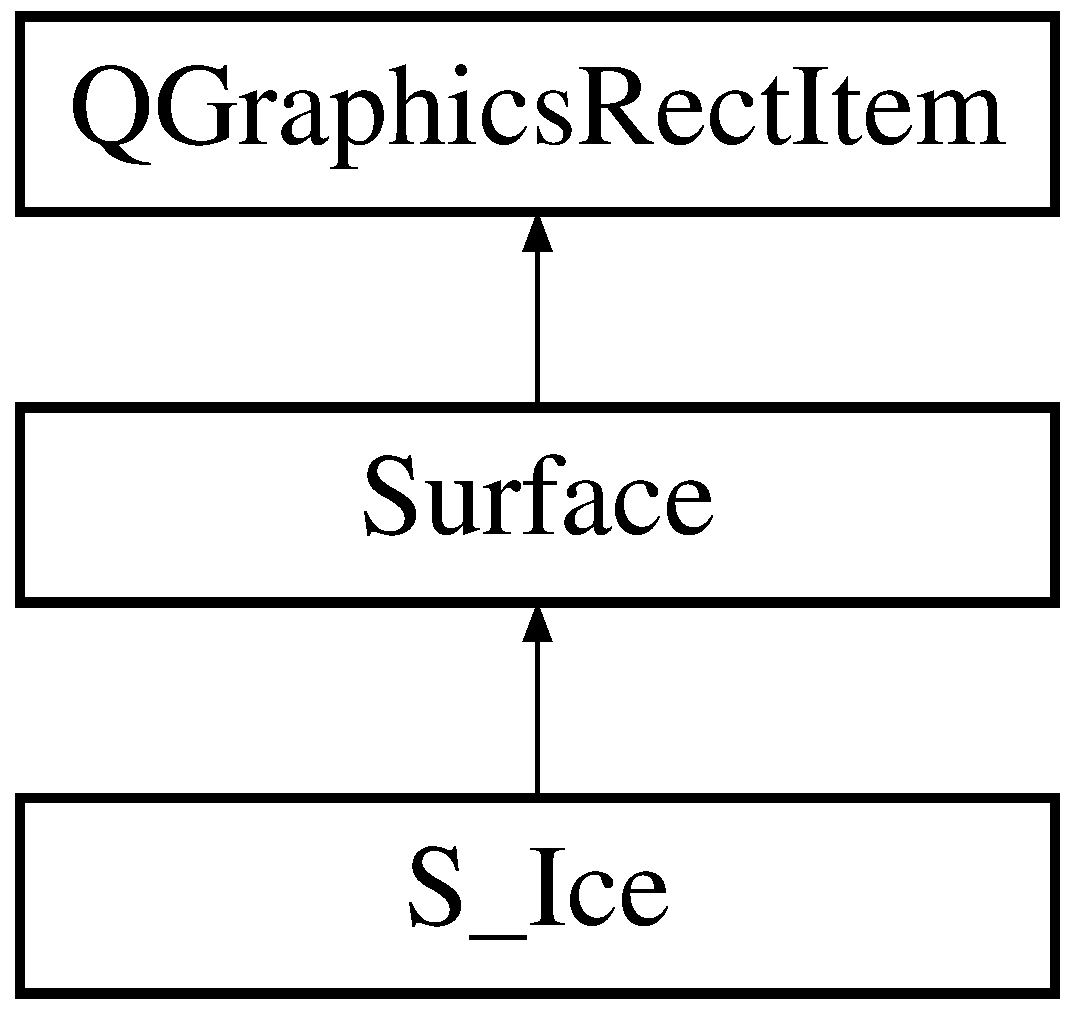
\includegraphics[height=3.000000cm]{class_s___ice}
\end{center}
\end{figure}
\subsection*{Public Member Functions}
\begin{DoxyCompactItemize}
\item 
\hyperlink{class_s___ice_a3a1fdb0204964dfee672629d22cd0e76}{S\+\_\+\+Ice} (int xpos, int ypos, Q\+Graphics\+Item $\ast$parent=0)
\begin{DoxyCompactList}\small\item\em Constructor with position setup. \end{DoxyCompactList}\item 
\hyperlink{class_s___ice_a17b24abf85ec0bd466971675b657f856}{S\+\_\+\+Ice} (Q\+Graphics\+Item $\ast$parent=0)
\begin{DoxyCompactList}\small\item\em Constructor without position setup. \end{DoxyCompactList}\end{DoxyCompactItemize}


\subsection{Detailed Description}
Ice Surface. 

Specific design. \begin{DoxyAuthor}{Author}
Claret Romain, \href{mailto:romain.claret@rocla.ch}{\tt romain.\+claret@rocla.\+ch} 

Divernois Margaux, \href{mailto:margaux.divernois@gmail.com}{\tt margaux.\+divernois@gmail.\+com} 

Visinand Steve, \href{mailto:visinandst@gmail.com}{\tt visinandst@gmail.\+com} 
\end{DoxyAuthor}
\begin{DoxyCopyright}{Copyright}
Custom License + N\+D\+A 
\end{DoxyCopyright}
\begin{DoxyVersion}{Version}
1.\+0 
\end{DoxyVersion}
\begin{DoxyDate}{Date}
27 January 2015 
\end{DoxyDate}


\subsection{Constructor \& Destructor Documentation}
\hypertarget{class_s___ice_a3a1fdb0204964dfee672629d22cd0e76}{}\index{S\+\_\+\+Ice@{S\+\_\+\+Ice}!S\+\_\+\+Ice@{S\+\_\+\+Ice}}
\index{S\+\_\+\+Ice@{S\+\_\+\+Ice}!S\+\_\+\+Ice@{S\+\_\+\+Ice}}
\subsubsection[{S\+\_\+\+Ice}]{\setlength{\rightskip}{0pt plus 5cm}S\+\_\+\+Ice\+::\+S\+\_\+\+Ice (
\begin{DoxyParamCaption}
\item[{int}]{xpos, }
\item[{int}]{ypos, }
\item[{Q\+Graphics\+Item $\ast$}]{parent = {\ttfamily 0}}
\end{DoxyParamCaption}
)}\label{class_s___ice_a3a1fdb0204964dfee672629d22cd0e76}


Constructor with position setup. 


\begin{DoxyParams}{Parameters}
{\em xpos} & set the postion on the x-\/axis \\
\hline
{\em ypos} & set the postion on the y-\/axis \\
\hline
{\em parent} & Q\+Graphics\+Item parent \\
\hline
\end{DoxyParams}
\hypertarget{class_s___ice_a17b24abf85ec0bd466971675b657f856}{}\index{S\+\_\+\+Ice@{S\+\_\+\+Ice}!S\+\_\+\+Ice@{S\+\_\+\+Ice}}
\index{S\+\_\+\+Ice@{S\+\_\+\+Ice}!S\+\_\+\+Ice@{S\+\_\+\+Ice}}
\subsubsection[{S\+\_\+\+Ice}]{\setlength{\rightskip}{0pt plus 5cm}S\+\_\+\+Ice\+::\+S\+\_\+\+Ice (
\begin{DoxyParamCaption}
\item[{Q\+Graphics\+Item $\ast$}]{parent = {\ttfamily 0}}
\end{DoxyParamCaption}
)}\label{class_s___ice_a17b24abf85ec0bd466971675b657f856}


Constructor without position setup. 


\begin{DoxyParams}{Parameters}
{\em parent} & Q\+Graphics\+Item to depend on \\
\hline
\end{DoxyParams}


The documentation for this class was generated from the following files\+:\begin{DoxyCompactItemize}
\item 
s\+\_\+ice.\+h\item 
s\+\_\+ice.\+cpp\end{DoxyCompactItemize}

\hypertarget{class_s___snow}{}\section{S\+\_\+\+Snow Class Reference}
\label{class_s___snow}\index{S\+\_\+\+Snow@{S\+\_\+\+Snow}}


Snow \hyperlink{class_surface}{Surface}.  




{\ttfamily \#include $<$s\+\_\+snow.\+h$>$}

Inheritance diagram for S\+\_\+\+Snow\+:\begin{figure}[H]
\begin{center}
\leavevmode
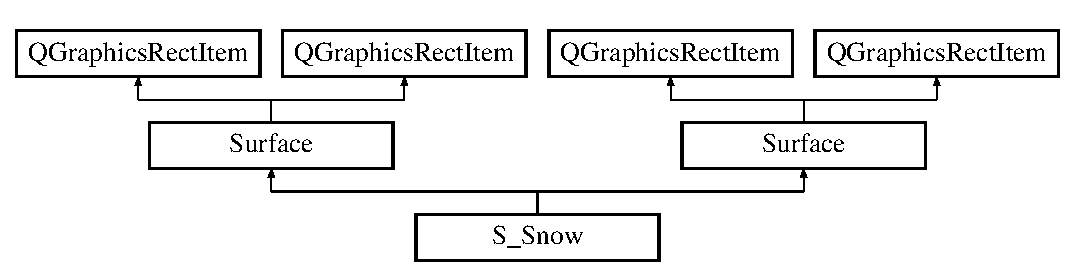
\includegraphics[height=3.000000cm]{class_s___snow}
\end{center}
\end{figure}
\subsection*{Public Member Functions}
\begin{DoxyCompactItemize}
\item 
\hypertarget{class_s___snow_a58b5eb7552b3082d105e9968acc7a9fb}{}{\bfseries S\+\_\+\+Snow} (int xpos, int ypos, Q\+Graphics\+Item $\ast$parent=0)\label{class_s___snow_a58b5eb7552b3082d105e9968acc7a9fb}

\item 
\hypertarget{class_s___snow_a19a17d0be19ecb0f85b1feff5aab697f}{}{\bfseries S\+\_\+\+Snow} (Q\+Graphics\+Item $\ast$parent=0)\label{class_s___snow_a19a17d0be19ecb0f85b1feff5aab697f}

\end{DoxyCompactItemize}


\subsection{Detailed Description}
Snow \hyperlink{class_surface}{Surface}. 

Specific design. \begin{DoxyAuthor}{Author}
Claret Romain, \href{mailto:romain.claret@rocla.ch}{\tt romain.\+claret@rocla.\+ch} 

Divernois Margaux, \href{mailto:margaux.divernois@gmail.com}{\tt margaux.\+divernois@gmail.\+com} 

Visinand Steve, \href{mailto:visinandst@gmail.com}{\tt visinandst@gmail.\+com} 
\end{DoxyAuthor}
\begin{DoxyCopyright}{Copyright}
Custom License + N\+D\+A 
\end{DoxyCopyright}
\begin{DoxyVersion}{Version}
1.\+0 
\end{DoxyVersion}
\begin{DoxyDate}{Date}
27 January 2015 
\end{DoxyDate}


The documentation for this class was generated from the following files\+:\begin{DoxyCompactItemize}
\item 
s\+\_\+snow.\+h\item 
s\+\_\+snow.\+cpp\end{DoxyCompactItemize}

\hypertarget{class_s___view_bloc_ennemi}{}\section{S\+\_\+\+View\+Bloc\+Ennemi Class Reference}
\label{class_s___view_bloc_ennemi}\index{S\+\_\+\+View\+Bloc\+Ennemi@{S\+\_\+\+View\+Bloc\+Ennemi}}
Inheritance diagram for S\+\_\+\+View\+Bloc\+Ennemi\+:\begin{figure}[H]
\begin{center}
\leavevmode
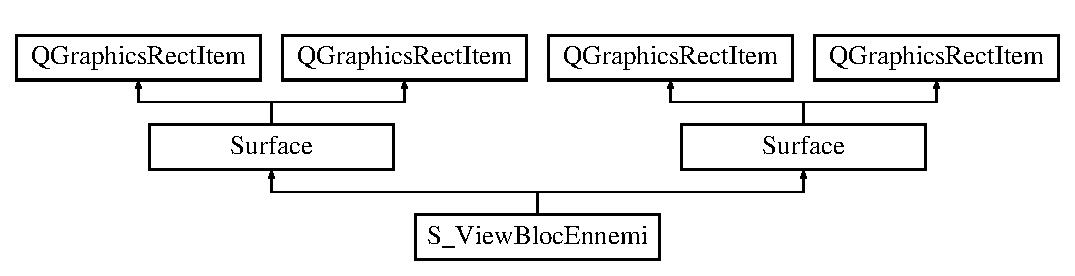
\includegraphics[height=3.000000cm]{class_s___view_bloc_ennemi}
\end{center}
\end{figure}
\subsection*{Public Member Functions}
\begin{DoxyCompactItemize}
\item 
\hypertarget{class_s___view_bloc_ennemi_a61ac9969081699f9cc22f89dcfdba2e6}{}{\bfseries S\+\_\+\+View\+Bloc\+Ennemi} (int ligne, int colonne, \hyperlink{class_ennemi}{Ennemi} $\ast$proprietaire, Q\+Graphics\+Item $\ast$parent=0)\label{class_s___view_bloc_ennemi_a61ac9969081699f9cc22f89dcfdba2e6}

\item 
\hypertarget{class_s___view_bloc_ennemi_af570c3ab5ad404591829ef8bbed13b08}{}int {\bfseries get\+Line} ()\label{class_s___view_bloc_ennemi_af570c3ab5ad404591829ef8bbed13b08}

\item 
\hypertarget{class_s___view_bloc_ennemi_ae843182fc545b9c84c22322873e499cd}{}int {\bfseries get\+Colonne} ()\label{class_s___view_bloc_ennemi_ae843182fc545b9c84c22322873e499cd}

\item 
\hypertarget{class_s___view_bloc_ennemi_a5aef2bd784ad1c7c180de4f5608a9624}{}bool {\bfseries is\+Actif} ()\label{class_s___view_bloc_ennemi_a5aef2bd784ad1c7c180de4f5608a9624}

\item 
\hypertarget{class_s___view_bloc_ennemi_a976bc517403eeef48f2e7d8bb67dfa99}{}void {\bfseries set\+Actif} (bool actif)\label{class_s___view_bloc_ennemi_a976bc517403eeef48f2e7d8bb67dfa99}

\item 
\hypertarget{class_s___view_bloc_ennemi_a3c6bb606eaf348d513caf0bfd73fd0aa}{}void {\bfseries pinguin\+On} ()\label{class_s___view_bloc_ennemi_a3c6bb606eaf348d513caf0bfd73fd0aa}

\item 
\hypertarget{class_s___view_bloc_ennemi_a930acab8e21620c59f18144230a9a33d}{}void {\bfseries bloc\+On} ()\label{class_s___view_bloc_ennemi_a930acab8e21620c59f18144230a9a33d}

\item 
\hypertarget{class_s___view_bloc_ennemi_a215944e297397346d3d5c0a08ae3d1fb}{}void {\bfseries set\+Style\+Pinguin\+On} ()\label{class_s___view_bloc_ennemi_a215944e297397346d3d5c0a08ae3d1fb}

\end{DoxyCompactItemize}
\subsection*{Public Attributes}
\begin{DoxyCompactItemize}
\item 
\hypertarget{class_s___view_bloc_ennemi_a85aabc73d2414af643c1d6e65a3384f5}{}\hyperlink{class_ennemi}{Ennemi} $\ast$ {\bfseries proprietaire}\label{class_s___view_bloc_ennemi_a85aabc73d2414af643c1d6e65a3384f5}

\end{DoxyCompactItemize}


The documentation for this class was generated from the following files\+:\begin{DoxyCompactItemize}
\item 
s\+\_\+viewblocennemi.\+h\item 
s\+\_\+viewblocennemi.\+cpp\end{DoxyCompactItemize}

\hypertarget{class_s___view_transition}{}\section{S\+\_\+\+View\+Transition Class Reference}
\label{class_s___view_transition}\index{S\+\_\+\+View\+Transition@{S\+\_\+\+View\+Transition}}


View Transition \hyperlink{class_surface}{Surface}.  




{\ttfamily \#include $<$s\+\_\+viewtransition.\+h$>$}

Inheritance diagram for S\+\_\+\+View\+Transition\+:\begin{figure}[H]
\begin{center}
\leavevmode
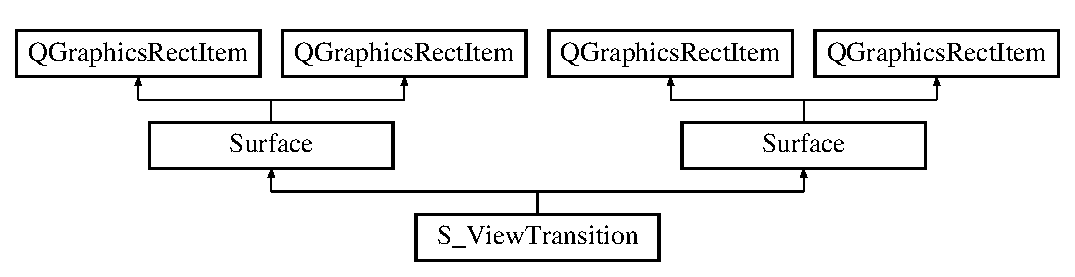
\includegraphics[height=3.000000cm]{class_s___view_transition}
\end{center}
\end{figure}
\subsection*{Public Member Functions}
\begin{DoxyCompactItemize}
\item 
\hypertarget{class_s___view_transition_a114168f77853ed98ff87d750f2982b39}{}{\bfseries S\+\_\+\+View\+Transition} (int xpos, int ypos, Q\+Graphics\+Item $\ast$parent=0)\label{class_s___view_transition_a114168f77853ed98ff87d750f2982b39}

\item 
\hypertarget{class_s___view_transition_a95dbe7a7f23bb8ed903ad8dff6f7ea6a}{}{\bfseries S\+\_\+\+View\+Transition} (Q\+Graphics\+Item $\ast$parent=0)\label{class_s___view_transition_a95dbe7a7f23bb8ed903ad8dff6f7ea6a}

\item 
\hypertarget{class_s___view_transition_ab6671a5c3df741a34c2cff8194c8c428}{}bool {\bfseries is\+End\+Level} ()\label{class_s___view_transition_ab6671a5c3df741a34c2cff8194c8c428}

\item 
\hypertarget{class_s___view_transition_afbfd78f5dcb2edb6b5444c4e2a73110a}{}void {\bfseries set\+Level\+End} (bool value)\label{class_s___view_transition_afbfd78f5dcb2edb6b5444c4e2a73110a}

\item 
\hypertarget{class_s___view_transition_af81ef15e45fb55bc71e3e81acb88971a}{}void {\bfseries set\+Needed\+Item} (Q\+String value)\label{class_s___view_transition_af81ef15e45fb55bc71e3e81acb88971a}

\item 
\hypertarget{class_s___view_transition_a9c7c1d53104949673f340c808682806d}{}Q\+String {\bfseries get\+Needed\+Item} ()\label{class_s___view_transition_a9c7c1d53104949673f340c808682806d}

\item 
\hypertarget{class_s___view_transition_a9f623ff7ddaa749fe32af0149e4dc7b7}{}bool {\bfseries is\+Needing\+Item} ()\label{class_s___view_transition_a9f623ff7ddaa749fe32af0149e4dc7b7}

\item 
\hypertarget{class_s___view_transition_a5926082bed3cb63fd6eea5e6d2cfb875}{}void {\bfseries set\+Nb\+Item} (int nb)\label{class_s___view_transition_a5926082bed3cb63fd6eea5e6d2cfb875}

\item 
\hypertarget{class_s___view_transition_aadf7b185d779366bc93d20856e0985c3}{}int {\bfseries get\+Nb\+Item} ()\label{class_s___view_transition_aadf7b185d779366bc93d20856e0985c3}

\item 
\hypertarget{class_s___view_transition_a7aa555ea153a02bc957cce590c7f0660}{}void {\bfseries set\+Next\+Level} (int nb)\label{class_s___view_transition_a7aa555ea153a02bc957cce590c7f0660}

\item 
\hypertarget{class_s___view_transition_aef44e5819f80ec0689175510a7d50c37}{}int {\bfseries get\+Next\+Level} ()\label{class_s___view_transition_aef44e5819f80ec0689175510a7d50c37}

\end{DoxyCompactItemize}


\subsection{Detailed Description}
View Transition \hyperlink{class_surface}{Surface}. 

This surface can move player\textquotesingle{}s view on the scene. It checks if the level is completed. Moves the player and changes the view to the next level is it\textquotesingle{}s complited. \begin{DoxyAuthor}{Author}
Claret Romain, \href{mailto:romain.claret@rocla.ch}{\tt romain.\+claret@rocla.\+ch} 

Divernois Margaux, \href{mailto:margaux.divernois@gmail.com}{\tt margaux.\+divernois@gmail.\+com} 

Visinand Steve, \href{mailto:visinandst@gmail.com}{\tt visinandst@gmail.\+com} 
\end{DoxyAuthor}
\begin{DoxyCopyright}{Copyright}
Custom License + N\+D\+A 
\end{DoxyCopyright}
\begin{DoxyVersion}{Version}
1.\+0 
\end{DoxyVersion}
\begin{DoxyDate}{Date}
27 January 2015 
\end{DoxyDate}


The documentation for this class was generated from the following files\+:\begin{DoxyCompactItemize}
\item 
s\+\_\+viewtransition.\+h\item 
s\+\_\+viewtransition.\+cpp\end{DoxyCompactItemize}

\hypertarget{structslide_bloc}{}\section{slide\+Bloc Struct Reference}
\label{structslide_bloc}\index{slide\+Bloc@{slide\+Bloc}}


Structure used in \hyperlink{class_gameboard}{Gameboard}.  




{\ttfamily \#include $<$gameboard.\+h$>$}

\subsection*{Public Attributes}
\begin{DoxyCompactItemize}
\item 
\hypertarget{structslide_bloc_a6fc7a4aca79032561e6d86f04b408695}{}\hyperlink{class_b___movable}{B\+\_\+\+Movable} $\ast$ {\bfseries sliding\+Movable}\label{structslide_bloc_a6fc7a4aca79032561e6d86f04b408695}

\item 
\hypertarget{structslide_bloc_adddf09c54543b518c768c0499f2db8b3}{}char {\bfseries sens}\label{structslide_bloc_adddf09c54543b518c768c0499f2db8b3}

\end{DoxyCompactItemize}


\subsection{Detailed Description}
Structure used in \hyperlink{class_gameboard}{Gameboard}. 

Used for blocks when they slides into a direction (\char`\"{}l\char`\"{}\+:left, \char`\"{}r\char`\"{}\+:right, \char`\"{}t\char`\"{}\+:top, \char`\"{}b\char`\"{}\+:bottom). \begin{DoxyRefDesc}{Todo}
\item[\hyperlink{todo__todo000007}{Todo}]integrate with D\+P Factory \end{DoxyRefDesc}


The documentation for this struct was generated from the following file\+:\begin{DoxyCompactItemize}
\item 
gameboard.\+h\end{DoxyCompactItemize}

\hypertarget{class_surface}{}\section{Surface Class Reference}
\label{class_surface}\index{Surface@{Surface}}
Inheritance diagram for Surface\+:\begin{figure}[H]
\begin{center}
\leavevmode
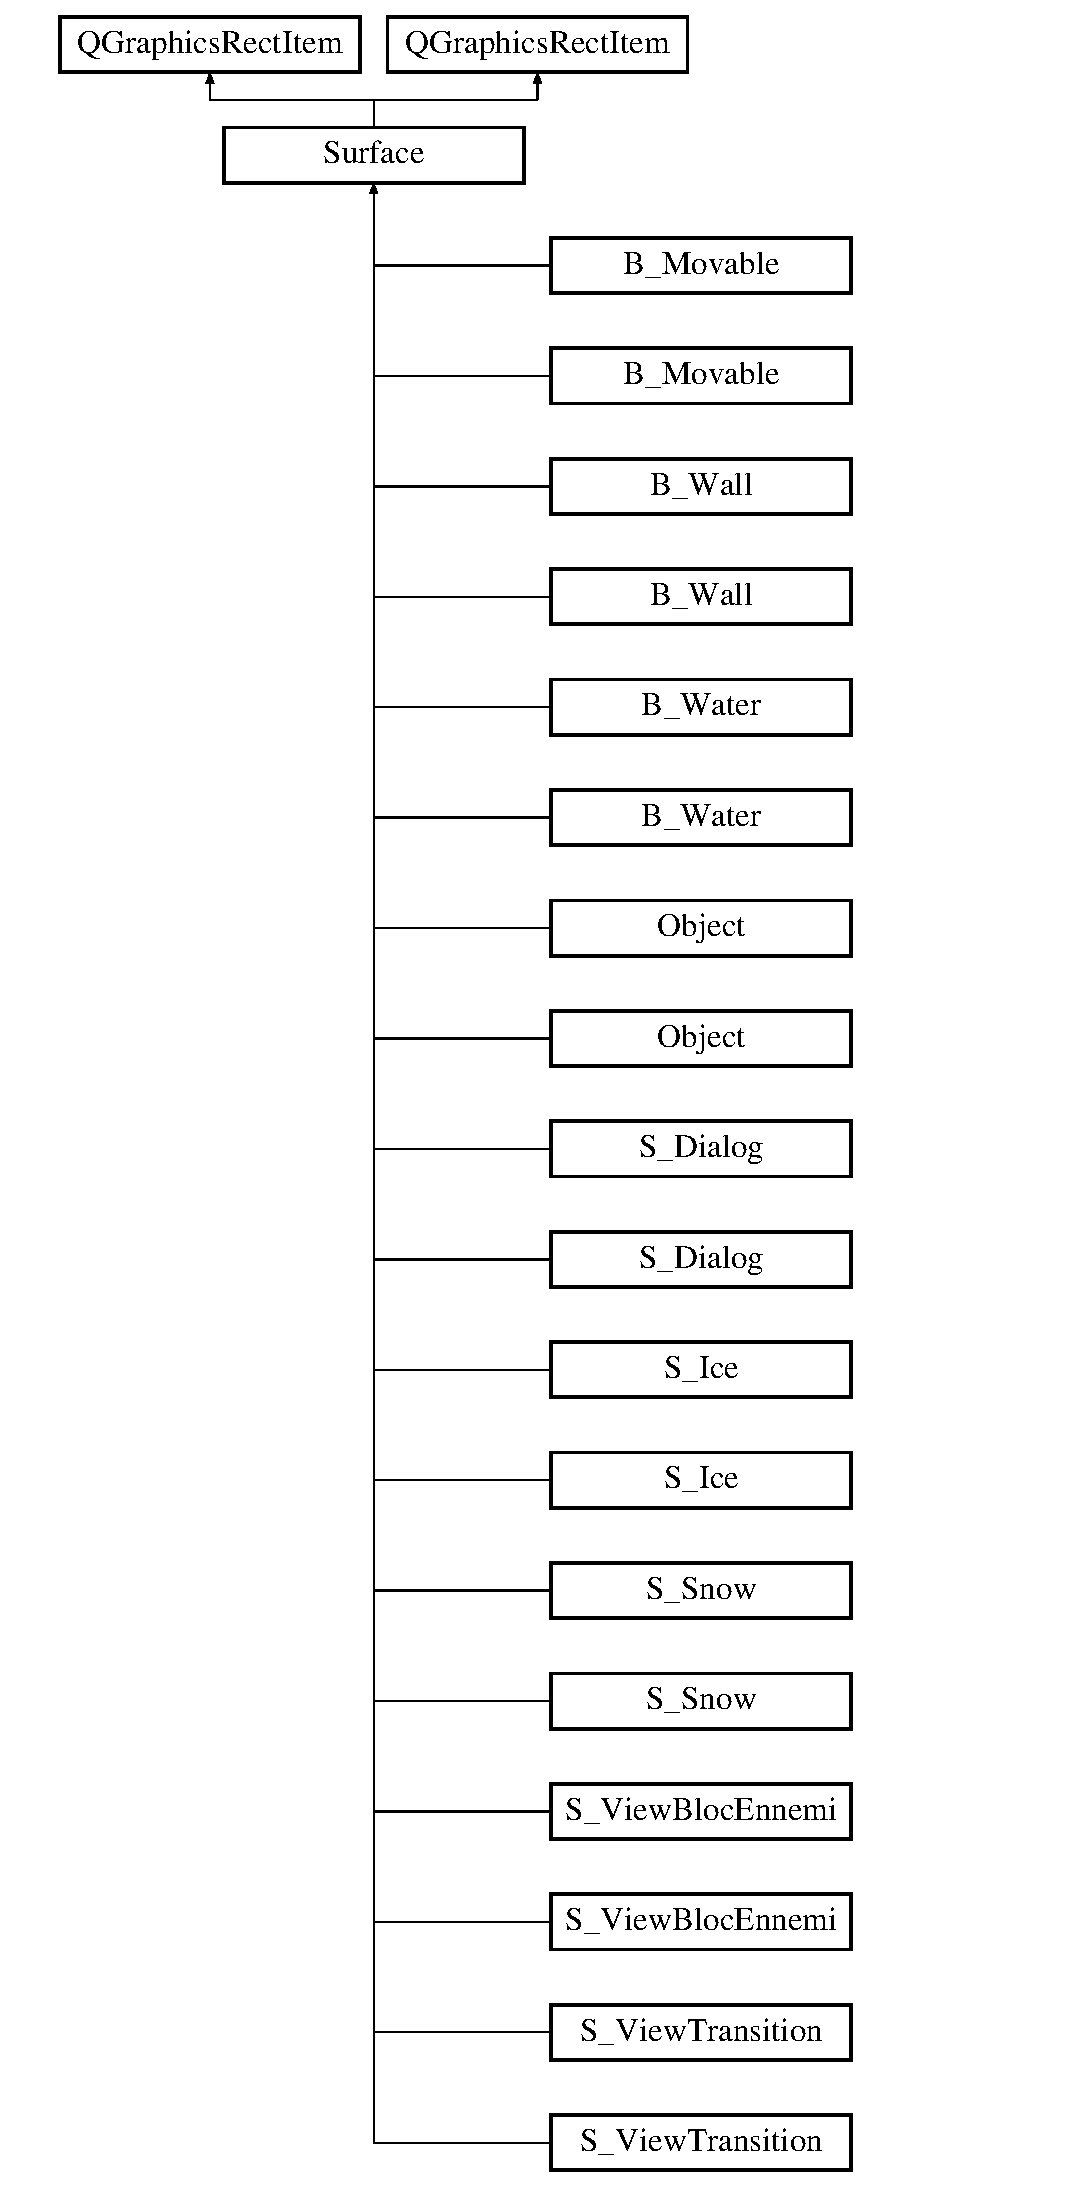
\includegraphics[height=11.000000cm]{class_surface}
\end{center}
\end{figure}
\subsection*{Public Member Functions}
\begin{DoxyCompactItemize}
\item 
\hypertarget{class_surface_ac03bea7e4e17982fd17f8a571035a6f0}{}{\bfseries Surface} (int xpos, int ypos, Q\+Graphics\+Item $\ast$parent=0)\label{class_surface_ac03bea7e4e17982fd17f8a571035a6f0}

\item 
\hypertarget{class_surface_a3e1af81e4723f854196608b966a86415}{}{\bfseries Surface} (int xpos, int ypos, int width, int height, Q\+Graphics\+Item $\ast$parent=0)\label{class_surface_a3e1af81e4723f854196608b966a86415}

\item 
\hypertarget{class_surface_a025ed38853ae95be3c6fe8814711ffc3}{}void {\bfseries set\+Pos} (int, int)\label{class_surface_a025ed38853ae95be3c6fe8814711ffc3}

\item 
\hypertarget{class_surface_ab63590ebca0d813b110aa286400eac72}{}void {\bfseries set\+Pos\+Pixel} (int, int)\label{class_surface_ab63590ebca0d813b110aa286400eac72}

\item 
\hypertarget{class_surface_acbdbf91a4cca74bb9da6c8a2fa932cd7}{}Q\+Point {\bfseries get\+Pos} ()\label{class_surface_acbdbf91a4cca74bb9da6c8a2fa932cd7}

\item 
\hypertarget{class_surface_ab7dd076ec71f2d6a63fe60f6c011786b}{}void {\bfseries set\+Color} (Q\+String brush\+Color)\label{class_surface_ab7dd076ec71f2d6a63fe60f6c011786b}

\end{DoxyCompactItemize}


The documentation for this class was generated from the following files\+:\begin{DoxyCompactItemize}
\item 
surface.\+h\item 
surface.\+cpp\end{DoxyCompactItemize}

\hypertarget{class_widget_dialog}{}\section{Widget\+Dialog Class Reference}
\label{class_widget_dialog}\index{Widget\+Dialog@{Widget\+Dialog}}
Inheritance diagram for Widget\+Dialog\+:\begin{figure}[H]
\begin{center}
\leavevmode
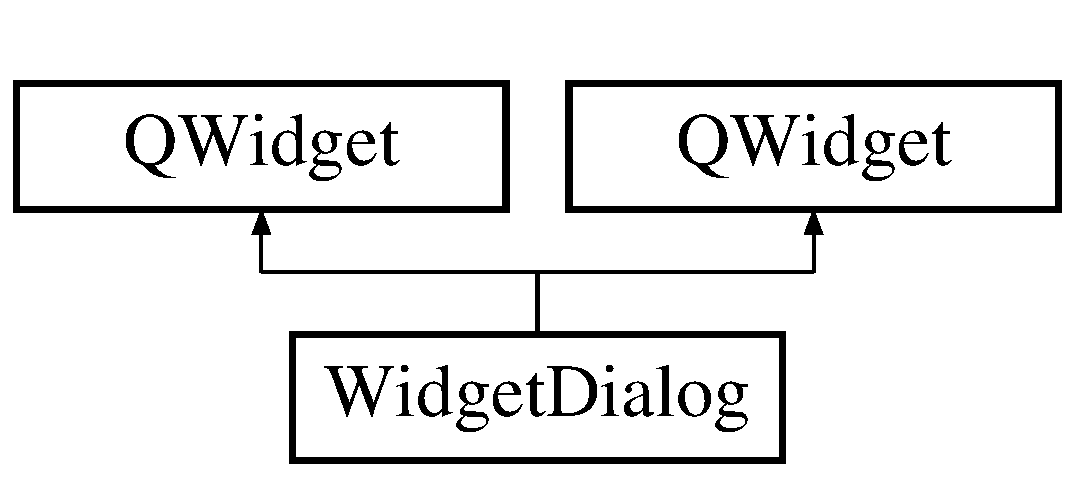
\includegraphics[height=2.000000cm]{class_widget_dialog}
\end{center}
\end{figure}
\subsection*{Public Member Functions}
\begin{DoxyCompactItemize}
\item 
\hypertarget{class_widget_dialog_aa282c5193c1318f92bd21fe77a3f66bb}{}{\bfseries Widget\+Dialog} (Q\+Widget $\ast$parent=0)\label{class_widget_dialog_aa282c5193c1318f92bd21fe77a3f66bb}

\item 
\hypertarget{class_widget_dialog_ad4ee3d228612e11780f73839db9150a9}{}void {\bfseries set\+Text} (Q\+String text, int type)\label{class_widget_dialog_ad4ee3d228612e11780f73839db9150a9}

\item 
\hypertarget{class_widget_dialog_ab904d7133d4de10e637cc48aac3a3ecc}{}Q\+String {\bfseries get\+Text} ()\label{class_widget_dialog_ab904d7133d4de10e637cc48aac3a3ecc}

\item 
\hypertarget{class_widget_dialog_aa3af6ec9a3e6dc42e82f86a851994614}{}void {\bfseries paint\+Event} (Q\+Paint\+Event $\ast$)\label{class_widget_dialog_aa3af6ec9a3e6dc42e82f86a851994614}

\end{DoxyCompactItemize}


The documentation for this class was generated from the following files\+:\begin{DoxyCompactItemize}
\item 
w\+\_\+dialog.\+h\item 
w\+\_\+dialog.\+cpp\end{DoxyCompactItemize}

\hypertarget{class_widget_life}{}\section{Widget\+Life Class Reference}
\label{class_widget_life}\index{Widget\+Life@{Widget\+Life}}


Diplay player\textquotesingle{}s life on the game.  




{\ttfamily \#include $<$w\+\_\+life.\+h$>$}

Inheritance diagram for Widget\+Life\+:\begin{figure}[H]
\begin{center}
\leavevmode
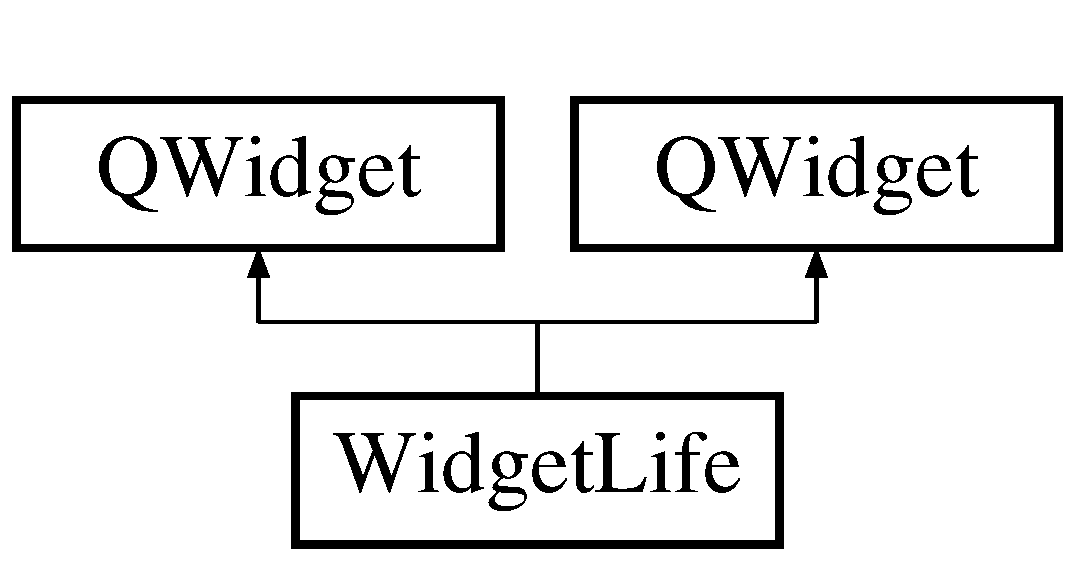
\includegraphics[height=2.000000cm]{class_widget_life}
\end{center}
\end{figure}
\subsection*{Public Member Functions}
\begin{DoxyCompactItemize}
\item 
\hypertarget{class_widget_life_a1d39aa69bd9872b67d0e5164f0bb1ca8}{}{\bfseries Widget\+Life} (Q\+Widget $\ast$parent=0)\label{class_widget_life_a1d39aa69bd9872b67d0e5164f0bb1ca8}

\item 
\hypertarget{class_widget_life_ab41e1bce66c7891a9f6f64d42d4f6055}{}void {\bfseries paint\+Event} (Q\+Paint\+Event $\ast$)\label{class_widget_life_ab41e1bce66c7891a9f6f64d42d4f6055}

\item 
\hypertarget{class_widget_life_af27cf30c08d8a7a85e29a0a3e2fae0b0}{}void {\bfseries update\+Hearts} (int value)\label{class_widget_life_af27cf30c08d8a7a85e29a0a3e2fae0b0}

\item 
\hypertarget{class_widget_life_a1d39aa69bd9872b67d0e5164f0bb1ca8}{}{\bfseries Widget\+Life} (Q\+Widget $\ast$parent=0)\label{class_widget_life_a1d39aa69bd9872b67d0e5164f0bb1ca8}

\item 
\hypertarget{class_widget_life_ab41e1bce66c7891a9f6f64d42d4f6055}{}void {\bfseries paint\+Event} (Q\+Paint\+Event $\ast$)\label{class_widget_life_ab41e1bce66c7891a9f6f64d42d4f6055}

\item 
\hypertarget{class_widget_life_af27cf30c08d8a7a85e29a0a3e2fae0b0}{}void {\bfseries update\+Hearts} (int value)\label{class_widget_life_af27cf30c08d8a7a85e29a0a3e2fae0b0}

\end{DoxyCompactItemize}


\subsection{Detailed Description}
Diplay player\textquotesingle{}s life on the game. 

Widget that shows on top of the game the amount of life left of the player. \begin{DoxyAuthor}{Author}
Claret Romain, \href{mailto:romain.claret@rocla.ch}{\tt romain.\+claret@rocla.\+ch} 

Divernois Margaux, \href{mailto:margaux.divernois@gmail.com}{\tt margaux.\+divernois@gmail.\+com} 

Visinand Steve, \href{mailto:visinandst@gmail.com}{\tt visinandst@gmail.\+com} 
\end{DoxyAuthor}
\begin{DoxyCopyright}{Copyright}
Custom License + N\+D\+A 
\end{DoxyCopyright}
\begin{DoxyVersion}{Version}
1.\+0 
\end{DoxyVersion}
\begin{DoxyDate}{Date}
27 January 2015 
\end{DoxyDate}


The documentation for this class was generated from the following files\+:\begin{DoxyCompactItemize}
\item 
gameboard.\+cpp\item 
w\+\_\+life.\+h\item 
w\+\_\+life.\+cpp\end{DoxyCompactItemize}

\hypertarget{class_widget_object}{}\section{Widget\+Object Class Reference}
\label{class_widget_object}\index{Widget\+Object@{Widget\+Object}}


Diplay player\textquotesingle{}s bag on the game.  




{\ttfamily \#include $<$w\+\_\+object.\+h$>$}

Inheritance diagram for Widget\+Object\+:\begin{figure}[H]
\begin{center}
\leavevmode
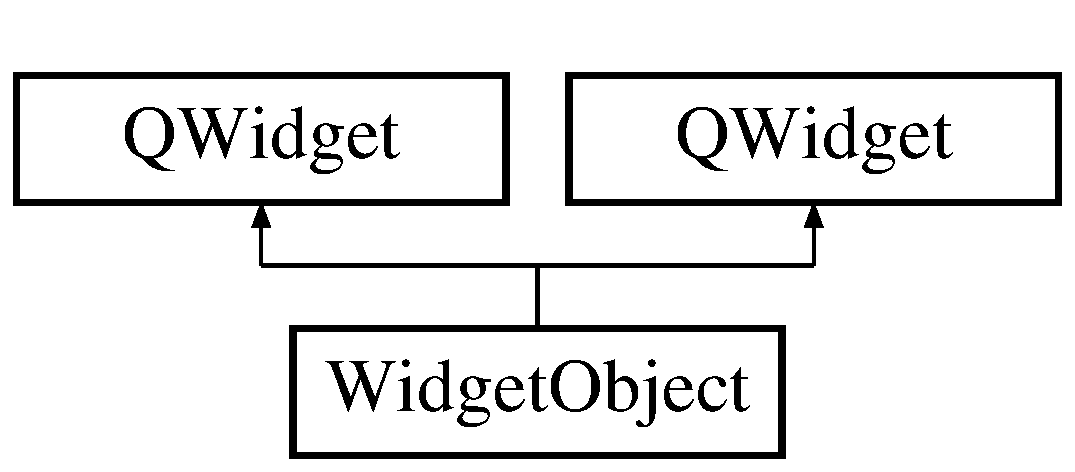
\includegraphics[height=2.000000cm]{class_widget_object}
\end{center}
\end{figure}
\subsection*{Public Member Functions}
\begin{DoxyCompactItemize}
\item 
\hypertarget{class_widget_object_a9afd6dc40c5f86a62260aab7da90240d}{}{\bfseries Widget\+Object} (Q\+Widget $\ast$parent=0)\label{class_widget_object_a9afd6dc40c5f86a62260aab7da90240d}

\item 
\hypertarget{class_widget_object_a60fa184f747fa815ff6b1604b16dfb01}{}void {\bfseries paint\+Event} (Q\+Paint\+Event $\ast$)\label{class_widget_object_a60fa184f747fa815ff6b1604b16dfb01}

\item 
\hypertarget{class_widget_object_ab94d05b6395226aa5e06a6a551c0ee47}{}void {\bfseries reload\+Object\+List} (Q\+List$<$ \hyperlink{class_object}{Object} $\ast$ $>$ object\+List)\label{class_widget_object_ab94d05b6395226aa5e06a6a551c0ee47}

\item 
\hypertarget{class_widget_object_a9afd6dc40c5f86a62260aab7da90240d}{}{\bfseries Widget\+Object} (Q\+Widget $\ast$parent=0)\label{class_widget_object_a9afd6dc40c5f86a62260aab7da90240d}

\item 
\hypertarget{class_widget_object_a60fa184f747fa815ff6b1604b16dfb01}{}void {\bfseries paint\+Event} (Q\+Paint\+Event $\ast$)\label{class_widget_object_a60fa184f747fa815ff6b1604b16dfb01}

\item 
\hypertarget{class_widget_object_ab94d05b6395226aa5e06a6a551c0ee47}{}void {\bfseries reload\+Object\+List} (Q\+List$<$ \hyperlink{class_object}{Object} $\ast$ $>$ object\+List)\label{class_widget_object_ab94d05b6395226aa5e06a6a551c0ee47}

\end{DoxyCompactItemize}


\subsection{Detailed Description}
Diplay player\textquotesingle{}s bag on the game. 

Widget that shows on top of the game the objects owned by the player. \begin{DoxyAuthor}{Author}
Claret Romain, \href{mailto:romain.claret@rocla.ch}{\tt romain.\+claret@rocla.\+ch} 

Divernois Margaux, \href{mailto:margaux.divernois@gmail.com}{\tt margaux.\+divernois@gmail.\+com} 

Visinand Steve, \href{mailto:visinandst@gmail.com}{\tt visinandst@gmail.\+com} 
\end{DoxyAuthor}
\begin{DoxyCopyright}{Copyright}
Custom License + N\+D\+A 
\end{DoxyCopyright}
\begin{DoxyVersion}{Version}
1.\+0 
\end{DoxyVersion}
\begin{DoxyDate}{Date}
27 January 2015 
\end{DoxyDate}


The documentation for this class was generated from the following files\+:\begin{DoxyCompactItemize}
\item 
gameboard.\+cpp\item 
w\+\_\+object.\+h\item 
w\+\_\+object.\+cpp\end{DoxyCompactItemize}

%--- End generated contents ---

% Index
\backmatter
\newpage
\phantomsection
\clearemptydoublepage
\addcontentsline{toc}{chapter}{Index}
\printindex

\end{document}
